% ============================================================================
%  VERIF-AI PROJECT VIVA PREPARATION HANDBOOK
%  Study material for Aniket Raj (230103030), B.Tech CSE (AI & DS), IIIT Senapati.
%  Every number in this handbook is taken from the project report, the repository's docs/ records and the source code.
%  Where something is not documented it is marked "Not documented" or "Pending verification".
%  Compile: latexmk -pdf Verif-AI_Project_Viva_Handbook.tex
% ============================================================================
\documentclass[11pt,a4paper]{report}
\usepackage[T1]{fontenc}
\usepackage{lmodern}
\usepackage[utf8]{inputenc}
\usepackage[a4paper,left=2.4cm,right=2.4cm,top=2.2cm,bottom=2.3cm]{geometry}
\usepackage{microtype}
\usepackage{graphicx}
\usepackage{xcolor}
\usepackage{array,booktabs,multirow,longtable,tabularx}
\usepackage{enumitem}
\usepackage{amsmath,amssymb}
\usepackage{fancyhdr}
\usepackage{needspace}
\usepackage{titlesec}
\usepackage{tikz}
\usetikzlibrary{arrows.meta,positioning,shapes.geometric,fit,calc,backgrounds}
\usepackage[skins,breakable]{tcolorbox}
\usepackage[hidelinks,pdftitle={Verif-AI Project Viva Preparation Handbook},pdfauthor={Aniket Raj}]{hyperref}

\definecolor{navy}{HTML}{0B2540}
\definecolor{teal}{HTML}{0F766E}
\definecolor{amber}{HTML}{B45309}
\definecolor{softgrey}{HTML}{F3F4F6}

\newcolumntype{L}[1]{>{\raggedright\arraybackslash}p{#1}}
\newcommand{\code}[1]{\texttt{\detokenize{#1}}}
\newcommand{\pfake}{\ensuremath{P_{\mathrm{fake}}}}

\setlength{\parindent}{0pt}
\setlength{\parskip}{0.45em}
\renewcommand{\arraystretch}{1.18}
\setlist{itemsep=0.15em,topsep=0.3em,parsep=0pt}
\setcounter{secnumdepth}{2}\setcounter{tocdepth}{2}
\sloppy\emergencystretch=2em

\titleformat{\chapter}[display]{\normalfont\huge\bfseries\color{navy}}{\Large Part \thechapter}{8pt}{\Huge}
\titlespacing*{\chapter}{0pt}{-8pt}{18pt}
\titleformat{\section}{\normalfont\Large\bfseries\color{navy}}{\thesection}{0.6em}{}
\titleformat{\subsection}{\normalfont\large\bfseries\color{teal}}{\thesubsection}{0.6em}{}

\pagestyle{fancy}\fancyhf{}
\fancyhead[L]{\small\color{navy}Verif-AI \,--\, Project Viva Preparation Handbook}
\fancyhead[R]{\small\leftmark}
\fancyfoot[C]{\small\thepage}
\renewcommand{\headrulewidth}{0.3pt}
\renewcommand{\chaptermark}[1]{\markboth{#1}{}}

% ---- boxes ----
\newtcolorbox{keybox}[1][Key idea]{colback=teal!6,colframe=teal,fonttitle=\bfseries\small,title={#1},boxrule=0.6pt,arc=2pt,left=6pt,right=6pt,top=4pt,bottom=4pt,breakable}
\newtcolorbox{warnbox}[1][Be careful]{colback=amber!8,colframe=amber,fonttitle=\bfseries\small,title={#1},boxrule=0.6pt,arc=2pt,left=6pt,right=6pt,top=4pt,bottom=4pt,breakable}
\newtcolorbox{sayit}[1][Say it like this]{colback=navy!5,colframe=navy,fonttitle=\bfseries\small,title={#1},boxrule=0.6pt,arc=2pt,left=6pt,right=6pt,top=4pt,bottom=4pt,breakable}

\begin{document}
\raggedbottom

% ============================ TITLE ============================
\begin{titlepage}
\centering
\vspace*{2.2cm}
{\Huge\bfseries\color{navy} Verif-AI\par}
\vspace{0.4cm}
{\LARGE\bfseries Project Viva Preparation Handbook\par}
\vspace{0.6cm}
{\large A Deep Learning-Based Framework for Face-Based Deepfake Detection and Forensic Analysis\par}
\vspace{2.2cm}
{\large Study material for\par}
\vspace{0.2cm}
{\Large\bfseries Aniket Raj\par}
{\large Roll No.\ 230103030 \,--\, B.Tech CSE (AI \& Data Science), Semester VII\par}
{\large Course CS4202 \,--\, Supervisor: Dr.\ Sunita Warjri, Assistant Professor, Department of CSE\par}
{\large Indian Institute of Information Technology Manipur\par}
\vfill
\begin{tcolorbox}[colback=softgrey,colframe=black!25,width=0.92\linewidth,left=8pt,right=8pt]
\small\textbf{How to use this handbook.} Parts 1--10 teach the whole project from the basics to the advanced details. Part 11 contains exactly 100 viva questions with answers.
Everything here follows the final project report and the experiment records in the repository. A number appears only if it is documented; otherwise it is marked
\emph{Not documented} or \emph{Pending verification}. Learn the \emph{ideas} and the \emph{honest limits} first; the numbers are easy to look up in the tables.
\end{tcolorbox}
\vspace{0.8cm}
{\small November 2026}
\end{titlepage}

\tableofcontents
\clearpage

% ============================================================================
\chapter{Project Introduction}
% ============================================================================

\section{What is Verif-AI?}
Verif-AI is a software system that looks at an \textbf{image or a video of a person's face} and reports whether the face looks \textbf{REAL}, \textbf{FAKE} or \textbf{INCONCLUSIVE}, together with
\emph{evidence} that a human can inspect. It is a complete application, not only a model:
\begin{itemize}
\item a \textbf{backend} (Python, FastAPI) that validates uploads, finds faces, runs the neural network and stores results;
\item a \textbf{deep-learning model} (PyTorch): a two-stream network built from two EfficientNet-B0 feature extractors, one reading the ordinary colour image (RGB stream) and one reading a
high-pass ``noise residual'' of the image (SRM stream);
\item an \textbf{explanation module} (Grad-CAM heat-maps) that shows which regions influenced the RGB stream;
\item for video, \textbf{face tracking}, a score-over-time timeline, suspicious time ranges and stored evidence frames;
\item a \textbf{PDF forensic report} that records the verdict, the file hash, the model checkpoint hash and the limitations;
\item a \textbf{web dashboard} (React + TypeScript) with upload, result viewers, history and deletion.
\end{itemize}

\begin{keybox}[One-sentence definition]
Verif-AI is a face-focused deepfake detector and forensic-evidence tool: it scores faces with a two-stream EfficientNet-B0 network, explains the score with Grad-CAM, summarises videos over time,
and produces a downloadable report --- while stating clearly that its score is a model output, not proof.
\end{keybox}

\section{What problem does it solve?}
Photographs and video used to be treated as informal evidence of identity and events. Generative models (GANs, face-swapping tools, diffusion models) can now create or alter faces so well that
people cannot reliably tell. This causes three practical problems:
\begin{enumerate}
\item \textbf{Detection:} given a face crop, estimate whether it shows a photographed face or a generated or manipulated one.
\item \textbf{Evidence:} a bare ``fake'' verdict is not enough for a reviewer; they need to see which face, which frames, what the model looked at, and which model and file were involved.
\item \textbf{Honesty and privacy:} neural scores are not probabilities, detectors are exposed to shortcuts, and uploaded media is personal data. A responsible tool must say ``inconclusive'' when it cannot decide and delete uploads after use.
\end{enumerate}

\section{Why was this project chosen?}
The project started from an earlier research prototype (a Forensic-Net style notebook with an RGB and an SRM stream, reporting very high accuracy on one dataset). When that prototype's
checkpoint was evaluated on independent, identity-disjoint data, it performed at chance level. This made the central motivation of the project concrete:
\emph{a detector is only as trustworthy as the evidence about where it fails}. Verif-AI therefore (i) rebuilt the system as a clean, tested software package, (ii) trained and evaluated models under a
leakage-controlled protocol, and (iii) documented failures --- for example the failure on genuine video --- instead of hiding them.

\begin{warnbox}[Be honest about the prototype]
The earlier prototype's README claimed 99.2\% accuracy on Celeb-DF-v2. In this project that claim \textbf{could not be reproduced}: on identity-disjoint DeepFakeFace data the original checkpoint scored accuracy
0.503/0.511/0.507 (validation / internal test / cross-generator) with ROC-AUC 0.427/0.443/0.499, i.e.\ chance level. Never quote the old 99.2\% as a result of this project.
\end{warnbox}

\section{What are deepfakes?}
A \textbf{deepfake} is synthetic or manipulated media (image, video, audio) created or altered by deep-learning methods so that it looks authentic. In this project three kinds of face manipulation matter:
\begin{description}
\item[Face swap.] The face of person A is replaced by the face of person B in an image or video (e.g.\ InsightFace swaps in DeepFakeFace; the face-swap method used for Celeb-DF).
\item[Inpainting / editing.] Part of an image (the face region) is regenerated by a model such as Stable Diffusion inpainting.
\item[Fully synthetic faces.] A generator creates a face that never existed: GANs (e.g.\ StyleGAN) and diffusion models (e.g.\ Stable Diffusion text-to-image).
\end{description}

\section{Why is deepfake detection important?}
Fabricated faces can be used for fraud, impersonation, harassment, disinformation and for undermining genuine evidence (``liar's dividend''). At the same time, a \emph{wrong accusation} (calling a genuine
video fake) is also harmful. That is why this project reports both false positives and false negatives, never presents a score as a probability, and says ``Model-based evidence, not proof''.

\section{Objectives, scope and limitations}
\textbf{Objectives (from the report).}
\begin{enumerate}[label=O\arabic*.]
\item Re-implement the two-stream detector as a clean, tested software package with identical preprocessing at training time and inference time.
\item Train and evaluate models under identity-disjoint splits, duplicate removal, validation-only model selection and a clear separation of internal and cross-generator results.
\item Provide explainable output: Grad-CAM heat-maps, video timelines, face tracks, evidence frames and a PDF report, through an API and a web dashboard, with privacy-preserving handling of uploads.
\item Investigate honestly where the model fails (genuine video) and document the cause and the limits of every claim.
\item Deploy a public demonstration (static frontend, hosted API) and state its restrictions truthfully.
\end{enumerate}

\textbf{Scope.} Educational demonstration, exploratory review of suspicious \emph{face} media, and a research platform for studying detector generalisation.

\textbf{What the project does \emph{not} claim.}
\begin{itemize}
\item It is not a general detector of AI-generated images or videos, and it does not analyse audio, scenes or non-face content.
\item It does not establish authorship or provenance; a REAL verdict is not proof of authenticity.
\item No result supports a claim of ``95\%'' (or any fixed) accuracy for modern AI-generated images or videos.
\item The public deployment is a restricted demonstration, \emph{not} a production service.
\end{itemize}

\section{Research gap, contributions and novelty}
\label{sec:hb-novelty}
Your advisor may ask: \emph{``Many deepfake detectors already exist. What have you actually built that is new?''} The honest answer has four parts.
\begin{keybox}[What you must NOT claim]
Verif-AI is \textbf{not} a new deep-learning architecture. EfficientNet, the SRM idea, MTCNN and Grad-CAM are not yours, and the two-stream RGB + SRM design comes from the earlier \textbf{Forensic-Net prototype by Lakshya Singh}.
\end{keybox}
\begin{description}
\item[Research gap.] The papers reviewed (FaceForensics++, Celeb-DF, MesoNet/Xception, Zhou et al.\ two-stream, Luo et al.\ high-frequency features, Face X-ray, G\"uera \& Delp and Masi et al.\ for video, Wang/Ojha/Corvi on generalisation) present \emph{methods and benchmark results}. A usable forensic tool also needs per-face evidence, video timelines, honest uncertainty, privacy, and an evaluation that separates unseen identities from unseen generators. The inherited prototype reported very high accuracy that could not be reproduced on independent data.
\item[Built on established research.] EfficientNet-B0 backbones (Tan \& Le 2019), SRM-style high-pass kernels (Fridrich \& Kodovsk\'y 2012), the two-stream idea (Zhou et al.\ 2017), MTCNN (Zhang et al.\ 2016), Grad-CAM (Selvaraju et al.\ 2017), ImageNet initialisation, AdamW, PyTorch and the public datasets.
\item[Research novelty (empirical only).] The production model was at chance on held-out Celeb-DF video; image sharpness is a measurable shortcut carried mainly by the noise stream; a per-quality-bin gate fails all four models although two pass the usual ROC-AUC screen; E4 trades DeepFakeFace detection for Celeb-DF/\code{modern\_test} performance and fails the frozen promotion rule.
\item[Engineering novelty.] Training-matched preprocessing (JPEG round-trip), strict checkpoint loading with hash recording, an INCONCLUSIVE band, atomic job storage, privacy-preserving deletion, memory-aware hosting mode, and a model registry (default / alternative / rollback) that labels every result.
\item[System-level integration.] One React + FastAPI application joining face detection, two-stream inference, Grad-CAM, face tracking, timelines, evidence frames, PDF reports, history/deletion and a hosted demonstration; the prototype analysed only the first frame of a file.
\item[Experimental contribution.] A reproducible, leakage-controlled, pre-registered evaluation of four models plus E3/E4 under a frozen promotion rule, reported separately for internal, cross-generator, video and \code{modern\_test} settings.
\end{description}
\begin{sayit}[Answer to ``What is unique about your project?'']
``It is not a new architecture. It is an end-to-end, inspectable forensic application built around a two-stream detector, together with an evaluation that exposes where the detector fails --- for example chance-level behaviour on genuine video, the image-sharpness shortcut and a per-quality gate --- and a model registry that records which model and checkpoint produced each result. The two-stream design itself comes from the Forensic-Net prototype and the cited research.''
\end{sayit}

\section{The research papers behind Verif-AI}
All 36 references of the report are listed with DOIs in the file \texttt{Research\_References\_and\_Novelty.md} (in the \texttt{report} folder). The ones you must be able to explain:
\begin{center}
\footnotesize
\begin{tabular}{|L{3.6cm}|L{6.6cm}|L{4.6cm}|}
\hline
\textbf{Paper} & \textbf{What it introduced} & \textbf{Where Verif-AI uses it}\\\hline
Tan \& Le, 2019 (ICML) & EfficientNet, compound scaling; B0 baseline & backbone of both streams\\\hline
Fridrich \& Kodovsk\'y, 2012 (IEEE TIFS) & Spatial Rich Model: high-pass residual filters for steganalysis & three fixed kernels of the noise stream\\\hline
Zhou et al., 2017 (CVPRW) & two-stream tampered-face detector & the two-stream idea\\\hline
Zhang et al., 2016 (IEEE SPL) & MTCNN face detection & face localisation\\\hline
Selvaraju et al., 2017 (ICCV) & Grad-CAM & heat-maps on the RGB stream\\\hline
R\"ossler et al., 2019 (ICCV) & FaceForensics++ benchmark & field background (not used for training)\\\hline
Li et al., 2020 (CVPR) & Celeb-DF dataset & Celeb-DF training/test data (within-dataset evidence)\\\hline
Song et al., 2023 (arXiv) & DeepFakeFace dataset & main training/test data\\\hline
Karras et al., 2019 (CVPR) & StyleGAN and the FFHQ dataset & real faces for E3/E4\\\hline
Luo et al., 2021; Li et al., 2020 & high-frequency features / blending boundary for generalisation & related work only\\\hline
G\"uera \& Delp, 2018; Masi et al., 2020 & recurrent video detectors & related work (different from our tracking approach)\\\hline
Wang 2020; Ojha 2023; Corvi 2023 & detection across generators & motivates internal vs.\ cross-generator reporting\\\hline
Geirhos et al., 2020; Guo et al., 2017 & shortcut learning; over-confident scores & sharpness finding; scores not probabilities\\\hline
\end{tabular}
\end{center}

% ============================================================================
\chapter{Complete Project Architecture}
% ============================================================================

\section{Overall system architecture}
Verif-AI has three tiers (Figure~\ref{fig:tiers}):
\begin{figure}[ht]
\centering
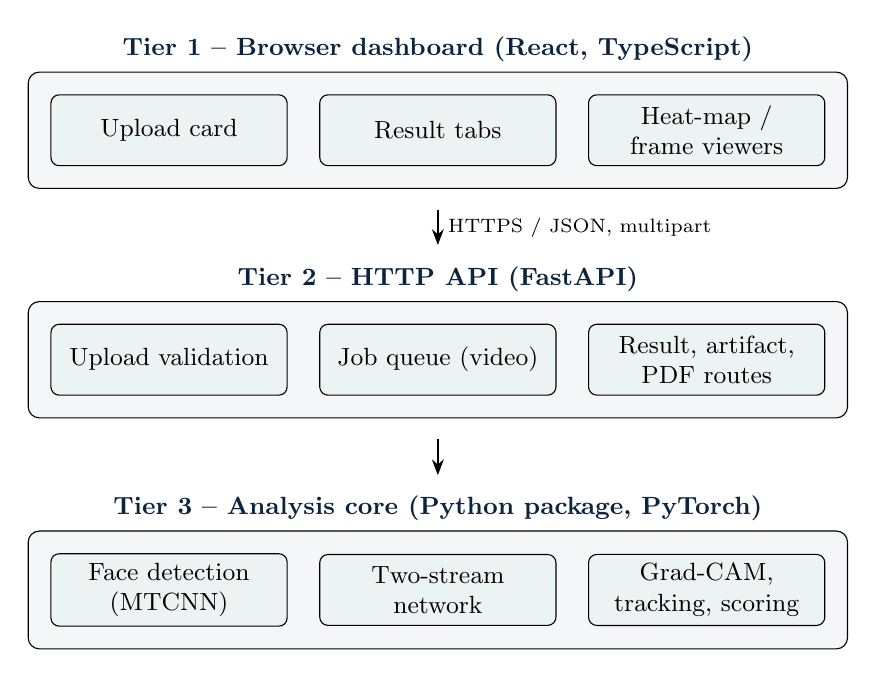
\begin{tikzpicture}[font=\small,
  box/.style={draw,rounded corners=3pt,minimum width=3.0cm,minimum height=0.9cm,align=center,fill=teal!8},
  tier/.style={draw,rounded corners=4pt,fill=navy!4,inner sep=8pt},
  arr/.style={-{Stealth[length=2mm]},thick}]
\node[box] (up) {Upload card};
\node[box,right=0.4cm of up] (res) {Result tabs};
\node[box,right=0.4cm of res] (vw) {Heat-map /\\frame viewers};
\begin{pgfonlayer}{background}\node[tier,fit=(up)(res)(vw),label={[navy,font=\small\bfseries]above:Tier 1 -- Browser dashboard (React, TypeScript)}] {};\end{pgfonlayer}
\node[box,below=2.0cm of up] (val) {Upload validation};
\node[box,right=0.4cm of val] (job) {Job queue (video)};
\node[box,right=0.4cm of job] (rt) {Result, artifact,\\PDF routes};
\begin{pgfonlayer}{background}\node[tier,fit=(val)(job)(rt),label={[navy,font=\small\bfseries]above:Tier 2 -- HTTP API (FastAPI)}] {};\end{pgfonlayer}
\node[box,below=2.0cm of val] (fd) {Face detection\\(MTCNN)};
\node[box,right=0.4cm of fd] (nn) {Two-stream\\network};
\node[box,right=0.4cm of nn] (gc) {Grad-CAM,\\tracking, scoring};
\begin{pgfonlayer}{background}\node[tier,fit=(fd)(nn)(gc),label={[navy,font=\small\bfseries]above:Tier 3 -- Analysis core (Python package, PyTorch)}] {};\end{pgfonlayer}
\draw[arr] ([yshift=-0.55cm]res.south)--node[right,font=\scriptsize]{HTTPS / JSON, multipart}([yshift=1.0cm]val.north -| res);
\draw[arr] ([yshift=-0.55cm]job.south)--([yshift=1.0cm]nn.north);
\end{tikzpicture}
\caption{The three tiers. The analysis core is a Python package with no web dependency, so the API, the training tools and the tests all share the same code.}
\label{fig:tiers}
\end{figure}

\begin{itemize}
\item \textbf{Frontend} (folder \code{frontend/}): React 18 + TypeScript, built with Vite, styled with Tailwind CSS 3. It never decides a verdict; it only displays what the API returns.
\item \textbf{Backend} (folder \code{backend/verifai/}): FastAPI application in \code{api/app.py}, analysis code in \code{model.py}, \code{faces.py}, \code{preprocess.py}, \code{scoring.py}, \code{image_pipeline.py},
\code{video_pipeline.py}, \code{explain.py}, \code{report.py}, \code{store.py}, \code{engine.py}.
\item \textbf{Training and research tools} (\code{backend/training/}) and \textbf{Kaggle notebook builders} (\code{kaggle/}), used offline on a Tesla T4 GPU.
\end{itemize}

\section{FastAPI backend and endpoints}
FastAPI is a Python web framework that builds an HTTP API with automatic request validation (Pydantic v2) and automatic documentation; it is served by Uvicorn. The endpoints (prefix \code{/api}):
\begin{center}
\small
\begin{tabular}{|l|l|p{7.2cm}|}
\hline
\textbf{Method} & \textbf{Path} & \textbf{Purpose}\\\hline
GET & \code{/health} & Liveness; whether the model is loaded\\\hline
GET & \code{/model} & Model card: name, checkpoint file, checkpoint SHA-256, thresholds, Grad-CAM availability\\\hline
POST & \code{/analyze/image} & Synchronous image analysis; returns the full result\\\hline
POST & \code{/analyze/video} & Starts a background job; returns HTTP 202 and an identifier\\\hline
GET & \code{/analyses} & Recent analyses (empty on the public deployment)\\\hline
GET & \code{/analyses/{id}/status} & Job state and progress\\\hline
GET & \code{/analyses/{id}} & Full result\\\hline
GET & \code{/analyses/{id}/report.pdf} & PDF forensic report\\\hline
GET & \code{/analyses/{id}/artifacts/{name}} & An evidence image (annotated image, face crop, heat-map, frame)\\\hline
DELETE & \code{/analyses/{id}} & Delete results and cancel a running job\\\hline
\end{tabular}
\end{center}

\section{Image analysis workflow, step by step}
\begin{enumerate}
\item The user selects an image. The dashboard checks type and size and shows a preview, then sends it as a multipart POST to \code{/api/analyze/image}.
\item The API \textbf{validates} the file: extension allow-list, size limit (default 15\,MB for images, 200\,MB for videos), pixel-count limit, and a real decoding check. The file is stored under a server-chosen name.
\item \textbf{Face detection (MTCNN).} Detection runs on a downscaled copy; boxes are scaled back to the original image. A face is kept if the detector confidence is $\ge 0.90$ and the shorter side is $\ge 32$\,px; faces below 96\,px are flagged as low resolution; at most 10 faces per image. If no face qualifies, the result is INCONCLUSIVE (``no usable face'') --- a result, not an error.
\item \textbf{Crop and normalise.} Each face is cropped with a margin of 20 px, resized to $224\times224$, passed through a \textbf{JPEG quality-95 round-trip} (because the training crops were stored as JPEG q95), and normalised with ImageNet mean and standard deviation.
\item \textbf{Scoring.} The two-stream network returns a raw sigmoid score $\pfake\in[0,1]$ for each face. The image score is the \textbf{maximum over faces}.
\item \textbf{Label.} With the fixed threshold 0.5: FAKE if $\pfake>0.5$, REAL otherwise; but if $|\pfake-0.5|<0.15$ the \emph{reporting} label becomes INCONCLUSIVE (the ``abstention band'').
\item \textbf{Evidence.} Grad-CAM heat-maps (when enabled), an annotated image with face boxes and face crops are stored; the result is saved as JSON with the file SHA-256, the checkpoint SHA-256 and the settings.
\item The \textbf{original upload is deleted} as soon as processing ends. The dashboard shows verdict, score, per-face cards and the heat-map viewer; the PDF can be downloaded and the analysis deleted.
\end{enumerate}

\section{Video analysis workflow, step by step}
Video can take a long time, so it runs as a \textbf{background job}: the POST returns an identifier immediately and the browser polls \code{/status}.
\begin{enumerate}
\item Sample frames at about 2 frames per second, at most 64 frames; corrupt frames are skipped.
\item Detect faces in each sampled frame and link them into \textbf{tracks} by bounding-box overlap (IoU).
\item Score all face crops in batches. The frame score is the maximum face score in the frame.
\item For each track with at least 3 observations take the \textbf{median} of its scores; the \textbf{video score is the maximum over tracks} (pooled fallback if no track is long enough). This aggregation rule was chosen \emph{a priori} and has \textbf{not been validated on labelled videos}.
\item Maximal runs of consecutive frames with score $>0.5$ become \textbf{suspicious time ranges}.
\item The \textbf{six highest-scoring frames} are stored as evidence, each with face boxes and a Grad-CAM heat-map for its top-scoring face; other frames show an honest ``not stored'' message.
\item The result tabs show the timeline, the frame viewer, face tracks, forensic evidence and the report.
\end{enumerate}

\section{How results are generated and displayed}
The result page is assembled only from fields of the API response: the verdict and raw score, a ``decisiveness'' value ($2|\pfake-0.5|$: low $<0.3$, moderate $<0.7$, high), the detector confidence, analysis settings, warnings and the limitation text.
The interface labels the number \emph{``model score, 0--1''} and never shows it as a percentage, because it is not a calibrated probability.

\section{Privacy and security design}
\begin{itemize}
\item Each analysis has a random 128-bit identifier; a result is reachable only by someone who knows it.
\item Uploads are deleted right after analysis (also on failure); results expire after a retention time (72\,h default) and can be deleted by the user.
\item The public deployment disables the global history list (\code{VERIFAI_PUBLIC_HISTORY=false}); the dashboard keeps only that browser's own list of identifiers.
\item CORS is restricted to the configured frontend origin.
\item \textbf{Not implemented:} authentication and rate limiting (stated as a limitation).
\end{itemize}

\begin{sayit}[Whiteboard summary of the data flow]
Browser $\rightarrow$ (multipart upload) $\rightarrow$ FastAPI validates $\rightarrow$ MTCNN finds faces $\rightarrow$ crop 224, JPEG q95, normalise $\rightarrow$ two-stream EfficientNet-B0 $\rightarrow$ raw sigmoid score $\rightarrow$ label with threshold 0.5 and $\pm0.15$ band
$\rightarrow$ Grad-CAM + stored evidence + JSON + PDF $\rightarrow$ dashboard; upload deleted. Video: same, plus frame sampling, tracking, median per track, maximum over tracks.
\end{sayit}

% ============================================================================
\chapter{Machine Learning and Deep Learning Fundamentals}
% ============================================================================

\section{AI, machine learning and deep learning}
\begin{description}
\item[Artificial intelligence (AI)] is the broad field of making machines do tasks that need intelligence (perception, language, decisions).
\item[Machine learning (ML)] is the part of AI in which a program \emph{learns patterns from data} instead of being given explicit rules. A model has parameters; training adjusts them to reduce an error measured on examples.
\item[Deep learning (DL)] is ML with \emph{many-layered neural networks} that learn useful features automatically (edges $\rightarrow$ textures $\rightarrow$ object parts). It is the standard tool for images.
\end{description}
Deepfake detection here is \textbf{binary classification}: input = a face image; output = a score for the class FAKE (label 1) versus REAL (label 0).

\section{Convolutional neural networks (CNNs)}
A CNN processes an image with small learnable filters (kernels, for example $3\times3$) that slide over the image. Each filter produces a \emph{feature map} that responds to a pattern. Stacking layers builds from low-level patterns (edges, textures) to high-level ones (face parts, blending artefacts).
Key components:
\begin{itemize}
\item \textbf{Convolution:} the sliding filter; weights are shared across positions, so the network needs far fewer parameters than a fully connected one.
\item \textbf{Non-linearity} (ReLU, SiLU/Swish): lets the network model complex functions.
\item \textbf{Pooling / stride:} reduces the spatial size. \textbf{Global average pooling} turns each feature map into one number (the average), giving a fixed-length vector regardless of image size.
\item \textbf{Batch normalisation:} stabilises and speeds up training.
\item \textbf{Fully connected (linear) layers:} combine the final features into the decision.
\end{itemize}

\section{Transfer learning}
Training a deep CNN from scratch needs a lot of data. \textbf{Transfer learning} starts from a network already trained on a large dataset (here ImageNet, about 1.28 million images) and \emph{fine-tunes} it on the new task.
The early layers already know generic visual features, so training is faster and needs less data. In this project the best runs were initialised from \textbf{ImageNet weights} (run B for the production model v2; also Models 2--4);
initialising from the old prototype checkpoint gave a lower validation ROC-AUC (0.9235 and 0.9284 versus 0.9477 for ImageNet initialisation).

\section{EfficientNet-B0}
EfficientNet (Tan and Le, ICML 2019) scales a CNN's \emph{depth, width and input resolution together} with a fixed compound coefficient. The smallest member, \textbf{B0}, has about 5.3 million parameters and reports 77.1\% ImageNet top-1 accuracy (published figure).
It is built from \textbf{MBConv} blocks (mobile inverted bottleneck with squeeze-and-excitation). Its last convolutional stage outputs a feature map with \textbf{1280 channels}; with $224\times224$ input this is a $7\times7$ grid, reduced by global average pooling to a \textbf{1280-dimensional vector}.
It was chosen because it is accurate for its size, so two copies fit comfortably on a CPU (the whole two-stream model has 11,972,954 parameters) and are fast to train on a single T4 GPU.

\begin{keybox}[Why EfficientNet-B0? (short answer)]
Good accuracy per parameter; small enough to run two parallel copies on a CPU; pretrained ImageNet weights are available for transfer learning; a 1280-dimensional feature vector is convenient for fusion.
\end{keybox}

\section{The two streams}
\subsection{RGB stream (spatial stream)}
The first stream is an EfficientNet-B0 without its classification layer. It reads the normal colour image and learns \emph{visible} inconsistencies: blending boundaries, lighting and texture inconsistencies, unnatural structure. Output: 1280-d vector.

\subsection{SRM noise stream}
The \textbf{Spatial Rich Model (SRM)} comes from image forensics (Fridrich and Kodovsk\'y, 2012): high-pass filters remove most image \emph{content} and leave the faint high-frequency \emph{noise residual}, in which traces of a generator or manipulation may remain.
In Verif-AI the second stream first passes the image through a \textbf{fixed (non-trainable) $3\times3$ convolution with three kernels}:
\begin{gather*}
K_1=\tfrac14\begin{pmatrix}-1&2&-1\\2&-4&2\\-1&2&-1\end{pmatrix},\qquad
K_2=\tfrac14\begin{pmatrix}-1&-1&-1\\-1&8&-1\\-1&-1&-1\end{pmatrix},\\[2pt]
K_3=\tfrac14\begin{pmatrix}0&-1&0\\-1&4&-1\\0&-1&0\end{pmatrix}.
\end{gather*}
Each kernel is applied to each of the R, G, B channels and the three channel outputs are summed, giving a 3-channel residual image. This residual is fed into a \emph{second} EfficientNet-B0. The kernels are constants (\code{requires_grad=False}) which keeps the stream's input independent of the training data.
The original rich model uses many more filters; Verif-AI uses three.

\begin{keybox}[Why an SRM stream?]
Generators and editing tools leave statistical traces in the high-frequency noise that are largely independent of the depicted content. The SRM stream looks at that noise while the RGB stream looks at what a person sees; the two views are complementary.
\end{keybox}

\begin{warnbox}[But the SRM stream also has a weakness (measured)]
Experiment E1 showed that image \emph{sharpness} is a dataset shortcut and that the noise stream carries much of the dependence on it (Spearman correlation of sharpness with the SRM-only score was $-0.36$ for real and $-0.52$ for fake faces for the production model on the DeepFakeFace internal test).
On Celeb-DF faces the production model's SRM-only score called 98.7\% of real faces fake. So ``SRM is good'' is \emph{not} an unconditional claim --- say it is \emph{designed} to expose generator traces, and that its behaviour was examined critically.
\end{warnbox}

\section{Two-stream architecture and feature fusion}
The two 1280-d vectors are \textbf{concatenated} (late fusion) into a 2560-d vector and passed through a small classification head:
\begin{gather*}
\underbrace{[\mathbf f_{RGB}\,;\,\mathbf f_{SRM}]}_{2560}\;\rightarrow\;\mathrm{Linear}(2560\!\to\!512)\rightarrow\mathrm{ReLU}\rightarrow\mathrm{Dropout}(0.5)\\
\rightarrow\;\mathrm{Linear}(512\!\to\!1)\rightarrow\text{logit}\rightarrow\sigma\rightarrow\pfake .
\end{gather*}
Late fusion means each stream computes its features separately and they are combined only at the end. Total: \textbf{11,972,954 parameters}. Because the head is joint, a stream cannot run alone; ``RGB-only'' and ``SRM-only'' scores in the experiments are \emph{conditional} scores obtained by replacing the other stream's features with the average of training crops.

\begin{figure}[ht]
\centering
\resizebox{\linewidth}{!}{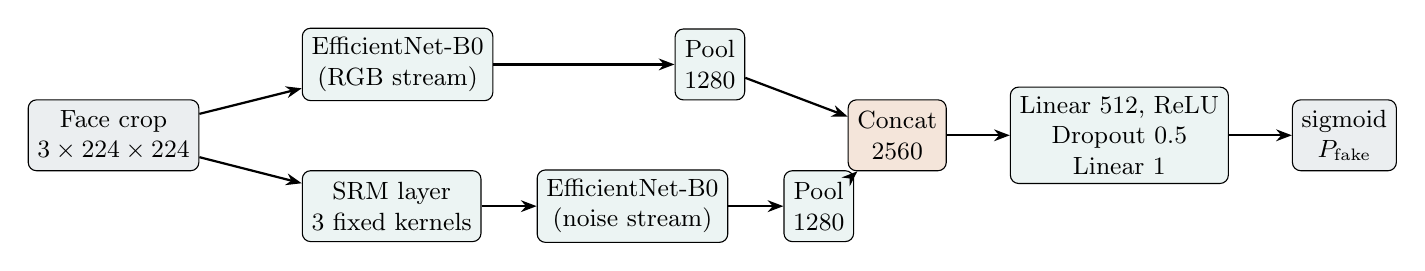
\begin{tikzpicture}[font=\small,
  n/.style={draw,rounded corners=3pt,minimum height=0.9cm,align=center,fill=teal!8},
  arr/.style={-{Stealth[length=2mm]},thick}]
\node[n,fill=navy!8] (in) {Face crop\\$3\times224\times224$};
\node[n,right=1.3cm of in,yshift=0.9cm] (b1) {EfficientNet-B0\\(RGB stream)};
\node[n,right=1.3cm of in,yshift=-0.9cm] (srm) {SRM layer\\3 fixed kernels};
\node[n,right=0.7cm of srm] (b2) {EfficientNet-B0\\(noise stream)};
\node[n,right=2.3cm of b1] (p1) {Pool\\1280};
\node[n,right=0.7cm of b2] (p2) {Pool\\1280};
\node[n,right=1.3cm of p1,yshift=-0.9cm,fill=amber!15] (cat) {Concat\\2560};
\node[n,right=0.8cm of cat] (hd) {Linear 512, ReLU\\Dropout 0.5\\Linear 1};
\node[n,right=0.8cm of hd,fill=navy!8] (out) {sigmoid\\$\pfake$};
\draw[arr](in)--(b1);\draw[arr](in)--(srm);\draw[arr](srm)--(b2);\draw[arr](b1)--(p1);\draw[arr](b2)--(p2);
\draw[arr](p1)--(cat);\draw[arr](p2)--(cat);\draw[arr](cat)--(hd);\draw[arr](hd)--(out);
\end{tikzpicture}}
\caption{The two-stream late-fusion network.}
\end{figure}

\section{Logits, sigmoid and thresholds}
The last linear layer outputs one real number, the \textbf{logit} $z$. The \textbf{sigmoid} $\sigma(z)=1/(1+e^{-z})$ squashes it into $(0,1)$. The result $\pfake$ is the model's \emph{score}; larger means ``more fake-like''.
A \textbf{threshold} turns the score into a decision: FAKE if $\pfake>0.5$. In Verif-AI the threshold is \textbf{fixed at 0.5 and never tuned on test data}. The \textbf{INCONCLUSIVE band} $|\pfake-0.5|<0.15$ is a reporting rule, not a change of the threshold.

\begin{warnbox}[Raw sigmoid score $\neq$ calibrated probability]
A \emph{calibrated} probability means: among all cases scored 0.9, about 90\% are really fake. A raw sigmoid output has no such guarantee; modern networks are usually over-confident (Guo et al., ICML 2017). Verif-AI never calibrated its scores, so 0.9 does \textbf{not} mean ``90\% likely fake'', and 0.000 or 1.000 does not mean certainty.
\end{warnbox}

\section{Loss, optimiser, epochs, batches}
\begin{itemize}
\item \textbf{Loss function:} a number that says how wrong the predictions are. Verif-AI uses \textbf{binary cross-entropy with logits} (BCE-with-logits) with a positive-class weight set from the training class counts (1.02 for the DeepFakeFace runs, 0.82 in E4).
For one example with label $y\in\{0,1\}$ and score $p$: $L=-[\,y\log p+(1-y)\log(1-p)\,]$; it is small when the model is confident and right, large when confident and wrong.
\item \textbf{Optimiser:} the algorithm that updates the weights to reduce the loss. Verif-AI uses \textbf{AdamW} (Adam with decoupled weight decay) with learning rate $10^{-4}$. A \textbf{learning-rate scheduler} (ReduceLROnPlateau) lowers the rate when validation stops improving; gradients are clipped at 5.
\item \textbf{Batch:} a group of examples processed together (batch size 32). \textbf{Epoch:} one full pass over the training set. Training ran for at most 15 epochs (12 for the later Celeb-DF experiments), with \textbf{early stopping} (patience 4 epochs on the validation selection metric).
\item \textbf{Training, validation and test sets:} \emph{training} data adjusts the weights; \emph{validation} data is used to choose when to stop and which checkpoint/model to keep; \emph{test} data is touched only at the end to report performance. Test data must never influence any decision.
\end{itemize}

\section{Overfitting, underfitting and generalisation}
\begin{description}
\item[Underfitting] the model is too simple or under-trained: poor accuracy even on training data.
\item[Overfitting] the model memorises training data (including its quirks) and does worse on new data: high training accuracy, lower validation/test accuracy. Remedies: more/better data, augmentation, dropout, early stopping, weight decay.
\item[Generalisation] performance on data the model has not seen. In deepfake detection there are \emph{several kinds} of ``unseen'': new \emph{identities}, new \emph{generators}, new \emph{datasets/footage}. This project measures them separately (internal vs.\ cross-generator vs.\ Celeb-DF).
\end{description}
Example from the project: Model 4 reaches training accuracy $\approx0.97$ and validation accuracy $\approx0.95$ in the later E4 experiment (validation only), but v2, which scores 0.875 on unseen identities, falls to 0.746 on an unseen generator --- a generalisation gap.

\section{Data augmentation and shortcuts}
\textbf{Augmentation} randomly alters training images (here: blur, down-up resampling, JPEG compression, noise, low light, applied \emph{class-blind}, i.e.\ identically to real and fake) so the model does not rely on fragile cues such as ``soft image $\Rightarrow$ fake''.
A \textbf{shortcut} (spurious cue) is a feature that predicts the label in the training data for the wrong reason. Experiment E1 found sharpness to be one: in DeepFakeFace, fakes are softer than real photographs (ROC-AUC of softness alone as a classifier of fake = 0.712 on training data, 0.680 on the internal test), and on the unseen generator the relation reverses (0.432).

% ============================================================================
\chapter{The Four Models}
% ============================================================================

\begin{keybox}[Exact names used in the project documents]
\textbf{Model 1 -- Production v2} (file \code{verifai_v2_best.pth}); \textbf{Model 2 -- DFF-only + quality augmentation}; \textbf{Model 3 -- DFF + Celeb-DF, no augmentation}; \textbf{Model 4 -- DFF + Celeb-DF + quality augmentation} (file \code{verifai_v3_celebdf_qa.pth}, the previous default and now an alternative). \textbf{E4} (file \code{verifai_e4_candidate.pth}) is the latest trained model and the default of the local examiner demonstration; v2 is the rollback model and the model served by the live site.
All four have the \emph{same architecture}; they differ only in \emph{training data} and \emph{augmentation}. They are compared in \code{docs/FOUR_MODEL_COMPARISON.md}. (The ``original prototype'' checkpoint is a separate baseline, not one of the four.)
\end{keybox}

\section{Why four models were compared}
After the production model v2 failed on genuine video, the team needed to know \emph{why} and \emph{what helps}. Two factors were changed one at a time:
(i) \textbf{adding Celeb-DF video frames} to the training data, and (ii) \textbf{adding class-blind quality augmentation}. This gives a $2\times2$ design: with/without Celeb-DF $\times$ with/without augmentation --- plus v2 as the baseline.

\begin{center}
\small
\begin{tabular}{|c|p{3.6cm}|p{3.4cm}|p{4.8cm}|}
\hline
\textbf{\#} & \textbf{Model} & \textbf{Training data} & \textbf{Selection (validation only)}\\\hline
1 & Production v2 & DeepFakeFace (DFF) & best validation ROC-AUC (epoch 9 of 13 run; 0.9477)\\\hline
2 & DFF-only + quality augmentation & DFF only, augmentation on 50\% of crops & best mean of clean and degraded validation ROC-AUC (epoch 15 = epoch cap)\\\hline
3 & DFF + Celeb-DF, no augmentation & DFF + Celeb-DF v2 frames (identity-disjoint) & same rule (epoch 4)\\\hline
4 & DFF + Celeb-DF + quality augmentation & same as 3, with augmentation & same rule (epoch 12 = epoch cap)\\\hline
\end{tabular}
\end{center}
All four start from \textbf{ImageNet} weights, use the same recipe (AdamW, $10^{-4}$, batch 32, BCE-with-logits, early-stopping patience 4) and the same seed.
Models 3 and 4 were trained on 2,315 DFF crops plus about 16,300 Celeb-DF crops (41 training identities); validation used 9 identities and testing used 9 \emph{other} identities.

\section{Results (same threshold 0.5, same test sets)}
FAKE is the positive class. ``Internal'' = unseen identities, generators seen in training. ``Cross-gen'' = unseen identities \emph{and} an unseen generator (text-to-image). ``Celeb-DF video'' = 147 held-out videos (91 real, 56 fake).

\begin{center}
\footnotesize\setlength{\tabcolsep}{4pt}
\begin{tabular}{|l|c|c|c|c|}
\hline
\textbf{Metric} & \textbf{1 v2} & \textbf{2} & \textbf{3} & \textbf{4}\\\hline
DFF internal -- accuracy & 0.875 & 0.856 & 0.852 & 0.835\\\hline
DFF internal -- ROC-AUC & 0.941 & 0.936 & 0.931 & 0.921\\\hline
DFF internal -- FPR / FNR & 0.140 / 0.110 & 0.151 / 0.138 & 0.127 / 0.170 & 0.130 / 0.201\\\hline
DFF cross-gen -- accuracy & 0.746 & 0.722 & 0.683 & 0.627\\\hline
DFF cross-gen -- ROC-AUC & 0.849 & 0.831 & 0.819 & 0.795\\\hline
DFF cross-gen -- FPR / FNR & 0.146 / 0.359 & 0.121 / 0.432 & 0.114 / 0.516 & 0.107 / 0.634\\\hline
Celeb-DF frames -- accuracy & 0.479 & 0.554 & 0.951 & 0.952\\\hline
Celeb-DF \textbf{video} -- accuracy & 0.483 & 0.578 & 0.973 & 0.980\\\hline
Celeb-DF video -- FPR (real called fake) & 0.604 (55/91) & 0.176 (16/91) & 0.044 (4/91) & 0.022 (2/91)\\\hline
Celeb-DF video -- FNR (fake called real) & 0.375 (21/56) & 0.821 (46/56) & 0.000 (0/56) & 0.018 (1/56)\\\hline
\end{tabular}
\end{center}
(Source: four-model comparison, 95\% Wilson/bootstrap intervals in the document; Celeb-DF numbers are \emph{within-dataset} evidence.)

\section{Strengths and weaknesses of each model}
\begin{description}
\item[Model 1 -- v2.] \textbf{Strength:} best on DeepFakeFace (0.875 internal, 0.746 cross-generator) and the best unseen-generator recall (64.1\% of text-to-image fakes detected). \textbf{Weakness:} at chance level on genuine and face-swap video (video accuracy 0.483; 55 of 91 real videos called fake). Cause: an image-quality shortcut; its SRM stream says FAKE for nearly all Celeb-DF faces.
\item[Model 2 -- DFF-only + augmentation.] \textbf{Strength:} more robust to blur/compression than v2. \textbf{Weakness:} still cannot separate real from fake on Celeb-DF video (FNR 0.821, ROC-AUC 0.516); its lower false-positive rate is \emph{not} a fix --- it just says REAL for nearly everything. Documented as \textbf{not recommended}.
\item[Model 3 -- DFF + Celeb-DF, no augmentation.] \textbf{Strength:} solves the Celeb-DF video problem (accuracy 0.973). \textbf{Weakness:} fragile under degradation (video accuracy falls to 0.844 under strong blur; FPR 0.132) and weaker on DeepFakeFace.
\item[Model 4 -- DFF + Celeb-DF + augmentation.] \textbf{Strength:} the best and most robust on Celeb-DF (video accuracy 0.980; 0.959--0.986 under every tested degradation). \textbf{Weakness:} the weakest on DeepFakeFace, especially the unseen generator (FNR 0.634: 63\% of text-to-image fakes pass as real).
\end{description}

\section{Which model is the default and why}
\textbf{E4 is the default model of the local examiner demonstration} (the local application loads \code{backend/models/verifai_e4_candidate.pth}, SHA-256 starting \code{0d553de9}); \textbf{Model 4} is an alternative and \textbf{v2} is the rollback model and the model served by the live website. The reasons for choosing E4 for the demonstration:
\begin{itemize}
\item It is the latest trained model and has the strongest held-out results on Celeb-DF video (0.980) and on \code{modern\_test} (0.983).
\item Compared with Model 4 it recovers part of the unseen-generator detection (DeepFakeFace cross-generator missed-fake rate 0.509 against 0.634).
\item The dashboard names it on the home page, in every result chip and in the PDF report, together with its status note.
\end{itemize}
\begin{warnbox}[Say this clearly]
E4 is the demonstration default by \textbf{owner decision}; it \textbf{did not pass} the project's frozen production-promotion rule (criterion 2: DeepFakeFace missed-fake rate 0.208 internal against a limit of 0.160, and 0.509 cross-generator against 0.409). v2 is still the best model on DeepFakeFace (0.875 / 0.746). Neither model reliably detects modern AI-generated photographs, and the \code{modern\_test} figure is not generator-disjoint.
E4 is \emph{not} deployed on the live website: its checkpoint is not in Git and the free 512\,MB host cannot hold it, so the live API still serves v2.
\end{warnbox}

\section{Quality-bin acceptance gate (stage 0)}
Overall accuracy hides quality-dependent failures, so a per-quality-bin gate with thresholds frozen \emph{before} any run was designed (G1: each stream separates the classes; G2: scores not correlated with sharpness within a class; G3: error rates do not vary across quality bins; G4: separation within bins), on validation data only. Synthetic controls validated the gate itself (a softness-only classifier must fail it).
\textbf{All four models failed the gate} (13, 9, 8 and 3 failed checks for Models 1, 2, 3, 4). Models 3 and 4 pass the simple ``ungated'' screen (ROC-AUC $\ge$ 0.90 on both clean validation sets) but fail the gate --- which shows the gate carries information that aggregate accuracy does not.
Disclosure: the gate thresholds were set while reading E1 results that included test splits, so independence from test data cannot be proved.

\section{Further experiments: E3 and E4}
\textbf{E3 (modern-generator data).} Real faces from FFHQ and synthetic faces from SFHQ plus the fake side of DeepDetect-2025 were added. Two candidates were trained: \textbf{E3A} (with quality augmentation) and \textbf{E3B} (without); the choice used validation only (E3A validation selection score 0.980 vs.\ 0.939). Results on the held-out \code{modern_test}: E3A accuracy 0.983 (FPR 0.014, FNR 0.019), E3B 0.981, but Model 4 only 0.328 and v2 0.326.
\textbf{But this is not generator-disjoint evidence:} the fakes in \code{modern_test} come from the same generator families as the training fakes and all its real faces are FFHQ, so an ``FFHQ-versus-generated'' shortcut cannot be excluded.
On the genuinely unseen generator (DeepFakeFace text2img) E3A is \emph{not} better than Model 4 (FNR 0.624 vs.\ 0.634) and clearly worse than v2 (0.359).

\textbf{The frozen promotion rule} (written before training). A candidate replaces the default only if \emph{all} hold:
\begin{enumerate}
\item \textbf{Celeb-DF video:} FPR $\le$ Model 4's FPR $+0.03$ \emph{and} accuracy $\ge0.95$;
\item \textbf{DeepFakeFace:} FNR $\le$ v2's FNR $+0.05$ \emph{and} FPR $\le0.20$, on both internal and cross-generator tests;
\item \textbf{modern\_test:} balanced accuracy $\ge$ Model 4's $+0.10$ with the confidence interval of the difference above 0.
\end{enumerate}
E3A passes criteria 1 (FPR 0.022 vs 0.011; accuracy 0.980) and 3 (balanced accuracy 0.984 vs 0.475) but \textbf{fails criterion 2} (internal FNR 0.230 vs.\ limit 0.160; cross-generator FNR 0.624 vs.\ limit 0.409). Therefore \textbf{E3A was not promoted and Model 4 remains the default}. (Model 4 itself would also fail criterion 2 --- the rule is about replacing the \emph{current} default by a better all-round model.)

\textbf{E4 (source-balanced variant).} E4 repeats every DeepFakeFace \emph{training} row four times (validation and test unchanged) in the E3A recipe, to test whether the small share of DeepFakeFace (about 5\% of training fakes) causes the loss of DeepFakeFace detection.
\textbf{Status: completed and verified.} The Kaggle run finished (12 of 12 epochs, 134.5 minutes, best epoch 12, validation selection score 0.9797; validation accuracy 0.954, ROC-AUC 0.990). Held-out test results (E4 / Model 4 / v2): DeepFakeFace internal accuracy 0.831 / 0.835 / 0.875 (FNR 0.208 / 0.201 / 0.110); DeepFakeFace cross-generator accuracy 0.688 / 0.627 / 0.746 (FNR 0.509 / 0.634 / 0.359); Celeb-DF video accuracy 0.980 / 0.980 / 0.476 (E4 FPR 0.022, FNR 0.018); \code{modern_test} accuracy 0.983 / 0.328 / 0.326. So repeating the DeepFakeFace rows recovered \emph{part} of the unseen-generator detection but not the internal test, and E4 \textbf{fails criterion 2 of the frozen rule} (internal FNR 0.208 vs.\ limit 0.160; cross-generator 0.509 vs.\ limit 0.409): E4 was \textbf{not promoted} and Model 4 remains the default. Same caveats as E3 (\code{modern_test} is not generator-disjoint; Celeb-DF is within-dataset; one run, one seed).

% ============================================================================
\chapter{Datasets}
% ============================================================================

\section{Overview}
\begin{center}
\small
\begin{tabular}{|L{2.3cm}|L{4.6cm}|L{3.9cm}|L{3.0cm}|}
\hline
\textbf{Dataset} & \textbf{What it is} & \textbf{Used for} & \textbf{Models}\\\hline
DeepFakeFace (DFF) & 30,000 real IMDB-WIKI photographs + 3$\times$30,000 fakes (inpainting, InsightFace face swap, text-to-image); published by Song et al.\ (arXiv:2309.02218), openrail licence & Training, validation and the two main tests (internal, cross-generator) & 1, 2, 3, 4 (and E3/E4)\\\hline
Celeb-DF v2 & Li et al., CVPR 2020: 590 real + 5,639 face-swap videos (+300 YouTube-real videos) & Training/validation/test of video-like faces & 3, 4 (and E3/E4)\\\hline
FFHQ & NVIDIA's 70,000 high-quality real face photographs (CC BY-NC-SA 4.0) & Real faces for E3 & E3A, E3B, E4\\\hline
SFHQ & Synthetic Faces High Quality (StyleGAN-generated, CC0) & Fake faces for E3 & E3A, E3B, E4\\\hline
DeepDetect-2025 & Collection of fakes from modern generators (real side not used) & Fake faces for E3 (face-filtered) & E3A, E3B, E4\\\hline
\end{tabular}
\end{center}
\textbf{Only a sample} of DeepFakeFace was used (a seeded, identity-disjoint sample fetched by HTTP range requests; the 5\,GB archives were never downloaded). For Celeb-DF, a third-party Kaggle copy (licence field ``unknown''; official terms: research use only) was used \emph{only inside a private notebook}; no frames left Kaggle.

\section{DeepFakeFace sample: sizes and splits}
Raw sample: 4,100 files (2,050 real--fake pairs). MTCNN found no face in 163 images (excluded); 8 images were removed as cross-split duplicates. Fake generators: \code{inpainting} (Stable Diffusion inpainting of the face region), \code{insight} (InsightFace face swap), \code{text2img} (Stable Diffusion v1.5 text-to-image). The real class is always the original IMDB-WIKI photograph (\code{wiki}).
\begin{center}
\small
\begin{tabular}{|l|p{4cm}|c|c|}
\hline
\textbf{Split} & \textbf{Purpose} & \textbf{Identities} & \textbf{Crops: real / fake}\\\hline
train & fitting (inpainting, insight) & 1,197 & 1,170 / 1,145 (total 2,315)\\\hline
val & early stopping and model selection (inpainting, insight) & 249 & 239 / 232 (471)\\\hline
test\_internal & unseen identities, \emph{seen} generators & 300 & 292 / 283 (575)\\\hline
test\_crossgen & unseen identities \emph{and unseen generator} (text2img) & 300 & 281 / 287 (568)\\\hline
\end{tabular}
\end{center}

\section{Celeb-DF v2 splits}
Videos were split \textbf{by identity}: 41 training identities, 9 validation identities and 9 \emph{different} test identities. A fake video was kept only if \emph{all} identities involved belong to the same split; YouTube-real videos were never used for testing.
Frames: 16 random frames per video (for the four-model comparison). Held-out test: 1,454 real + 896 fake face crops (frame level) and \textbf{147 videos (91 real, 56 fake)} at video level. (In the later E3 evaluation the Celeb-DF crops were re-extracted: 1,453 real / 895 fake; numbers differ slightly, e.g.\ v2 video accuracy 0.476 there against 0.483.)

\section{E3 data (modern generators)}
\begin{center}
\small
\begin{tabular}{|l|c|c|c|}
\hline
\textbf{Source (label)} & \textbf{Train} & \textbf{Validation} & \textbf{modern\_test}\\\hline
FFHQ (real) & 7,996 & 966 & 1,447\\\hline
SFHQ (fake) & 3,000 & 473 & 677\\\hline
DeepDetect fake & 8,997 & 880 & 2,202\\\hline
\end{tabular}
\end{center}
After face detection and near-duplicate removal (179 validation and 373 test crops removed because they were near-duplicates of training crops). DeepDetect has no per-image generator labels, so per-generator results are not available for it.
Two other candidate datasets (RealVsFake 162k and DeepFakeFusion-399K) were \textbf{excluded} after a provenance review (non-commercial or access-agreement sources behind ``open'' licence badges, overlap with the Celeb-DF test data, and format shortcuts).

\section{Preprocessing and augmentation}
\begin{enumerate}
\item MTCNN finds the largest face; crop with margin 20 px; resize to $224\times224$; \textbf{save as JPEG quality 95} (this is how the original training crops were stored, and inference reproduces it).
\item Normalise with the ImageNet mean and standard deviation.
\item \textbf{Quality augmentation} (Models 2 and 4; E3A/E4): with probability 0.5 per crop, apply a random class-blind degradation: Gaussian blur, down-up resampling, JPEG compression (quality 15--70), noise, or low-light with noise. Real and fake crops are treated identically.
\item Validation also reports ``clean'' and ``degraded'' ROC-AUC; the selection score for augmented runs is the \textbf{mean of clean and degraded validation ROC-AUC}.
\end{enumerate}

\section{How data leakage was avoided}
\begin{center}
\small
\begin{tabular}{|p{4.4cm}|p{6.2cm}|p{3.6cm}|}
\hline
\textbf{Risk} & \textbf{Control} & \textbf{Result}\\\hline
Same person in several splits & Split by identity; automatic check of identity and pair disjointness & 0 violations\\\hline
Real photo and its fake in different splits & Pair = same identity $\Rightarrow$ same split & 0 violations\\\hline
Duplicates across splits & SHA-256 (exact) and 64-bit difference hash (near) search; the item in the later split is dropped & 8 cross-split pairs removed (DFF); Hamming $\le3$ for E3\\\hline
Test used for selection & Early stopping and checkpoint choice on \texttt{val} only; the threshold is never tuned & by construction\\\hline
Same video in several splits & Group by identity / source video; cross-split fakes dropped & implemented\\\hline
\end{tabular}
\end{center}
The data-validation script aborts if it finds leakage. Remaining caveat: the stage-0 gate thresholds were set with knowledge of earlier test-split diagnostics (disclosed).

\section{Why these datasets and what are their limits}
\begin{itemize}
\item \textbf{DeepFakeFace:} openly available (openrail), ground truth known \emph{by construction} (real original vs.\ generated from it), contains an \emph{unseen-generator} split. \textbf{Limits:} generators are about 2023-era; one real source (IMDB-WIKI, celebrity photographs); fakes from one family of pipelines; demographic bias not characterised.
\item \textbf{Celeb-DF v2:} the standard challenging face-swap video benchmark; needed to study genuine video. \textbf{Limits:} one face-swap method and one kind of footage (YouTube celebrity clips), only 9 test identities and 147 test videos, third-party copy with unclear licence status. \textbf{Celeb-DF accuracy is within-dataset evidence only.}
\item \textbf{FFHQ/SFHQ/DeepDetect:} bring modern generators. \textbf{Limits:} \code{modern_test} shares generator families with training fakes and its real side is a single source (FFHQ).
\item \textbf{Not used:} FaceForensics++, DFDC, DeeperForensics (access agreements or competition rules); unofficial mirrors were deliberately not used.
\end{itemize}

% ============================================================================
\chapter{Training and Evaluation}
% ============================================================================

\section{The training pipeline}
\begin{enumerate}
\item \textbf{Prepare data:} sample/fetch, detect faces, crop, store as JPEG q95, build manifests with file hashes.
\item \textbf{Validate data:} identity/pair disjointness, duplicates, class balance, shortcut diagnostics (script aborts on leakage).
\item \textbf{Train on a Kaggle Tesla T4 GPU} (private notebooks; only checkpoints and metrics are exported): AdamW lr $10^{-4}$, batch 32, BCE-with-logits (positive weight from class counts: 1.02 for DeepFakeFace runs, 0.82 in E4), ReduceLROnPlateau, gradient clipping 5, $\le$15 epochs (12 for Models 3/4), early-stopping patience 4, seed 42. The v2 runs took 7--9 minutes each.
\item \textbf{Select on validation only:} v2 by validation ROC-AUC; augmented runs by the mean of clean and degraded validation ROC-AUC.
\item \textbf{Evaluate once on test splits} with the fixed threshold 0.5: accuracy, precision, recall, F1, ROC-AUC, PR-AUC, confusion matrices, FPR/FNR with confidence intervals, per generator, and under fixed degradations.
\item \textbf{Reproduce locally on CPU:} the v2 checkpoint was re-evaluated on CPU and matched the GPU run to every printed digit (val 0.8769/0.9477, internal 0.8748/0.9410, cross-gen 0.7465/0.8492).
\end{enumerate}

\section{The confusion matrix and the metrics}
Take FAKE as the \emph{positive} class.
\begin{center}
\begin{tabular}{|c|c|c|}
\hline
 & \textbf{Predicted REAL} & \textbf{Predicted FAKE}\\\hline
\textbf{Actually REAL} & TN (true negative) & FP (false positive)\\\hline
\textbf{Actually FAKE} & FN (false negative) & TP (true positive)\\\hline
\end{tabular}
\end{center}
\begin{itemize}
\item \textbf{TP:} fake correctly called fake. \textbf{TN:} real correctly called real. \textbf{FP:} real wrongly called fake (a genuine person accused). \textbf{FN:} fake wrongly called real (a manipulation missed).
\item $\text{Accuracy}=\dfrac{TP+TN}{TP+TN+FP+FN}$; $\ \text{Precision}=\dfrac{TP}{TP+FP}$; $\ \text{Recall (TPR)}=\dfrac{TP}{TP+FN}$; $\ F_1=\dfrac{2PR}{P+R}$.
\item $\text{FPR}=\dfrac{FP}{FP+TN}$ (real called fake); $\ \text{FNR}=\dfrac{FN}{FN+TP}$ (fake called real); balanced accuracy $=1-\dfrac{FPR+FNR}{2}$.
\item \textbf{ROC-AUC:} area under the ROC curve (TPR against FPR over \emph{all} thresholds). It is the probability that a random fake gets a higher score than a random real face: 0.5 = chance, 1.0 = perfect. It does not depend on the 0.5 threshold. \textbf{PR-AUC:} area under the precision--recall curve.
\end{itemize}

\begin{keybox}[Worked example: Production v2 on the DeepFakeFace internal test]
Confusion matrix: TN $=251$, FP $=41$, FN $=31$, TP $=252$ (total 575; 292 real, 283 fake).\\[2pt]
Accuracy $=(252+251)/575=503/575=0.8748$ (reported 0.875).\quad Precision $=252/(252+41)=252/293=0.860$.\quad Recall $=252/(252+31)=252/283=0.890$.\\
$F_1=2(0.860)(0.890)/(0.860+0.890)=0.875$.\quad FPR $=41/292=0.140$.\quad FNR $=31/283=0.110$.\quad Balanced accuracy $=1-(0.140+0.110)/2=0.875$.
\end{keybox}

\section{Validation versus test, and how to read the results}
\begin{itemize}
\item \textbf{Validation} data guided the choice of the checkpoint and the run, so validation numbers are \emph{optimistic by construction} (v2: accuracy 0.877, ROC-AUC 0.948).
\item \textbf{Test} data was used only for final reporting (v2 internal: 0.875 / 0.941; cross-generator: 0.746 / 0.849).
\item \textbf{Training} accuracy is measured on the data the weights were fitted on; a large gap between training and test accuracy signals overfitting.
\item Always say \emph{which} test: \textbf{internal} (unseen identities, seen generators) is easier; \textbf{cross-generator} measures an unseen generator; \textbf{Celeb-DF} is within-dataset. Do not average them into one ``accuracy''.
\item Intervals: Wilson 95\% intervals for rates; grouped bootstrap (by identity) for ROC-AUC.
\end{itemize}

\section{The documented results at a glance}
\textbf{Production v2 (Model 1) on DeepFakeFace} (95\% bootstrap intervals in the report):
\begin{center}
\small
\begin{tabular}{|l|c|c|c|c|c|c|}
\hline
\textbf{Split} & \textbf{Acc} & \textbf{Prec} & \textbf{Recall} & \textbf{F1} & \textbf{ROC-AUC} & \textbf{FPR / FNR}\\\hline
Validation (selection) & 0.877 & 0.843 & 0.922 & 0.881 & 0.948 & 0.167 / 0.078\\\hline
Internal test & 0.875 & 0.860 & 0.890 & 0.875 & 0.941 & 0.140 / 0.110\\\hline
Cross-generator test & 0.746 & 0.818 & 0.641 & 0.719 & 0.849 & 0.146 / 0.359\\\hline
\end{tabular}
\end{center}
Per generator (internal): inpainting detected 91.5\%, insight (face swap) 86.6\%, real photographs accepted as REAL 85.9\%; unseen text2img detected only 64.1\%.
Original prototype checkpoint, same data: accuracy $\approx0.51$, ROC-AUC $\approx0.44$--$0.50$ (chance).

\textbf{Model 4 (alternative):} DFF internal accuracy 0.835 / ROC-AUC 0.921; DFF cross-generator accuracy 0.627 / ROC-AUC 0.795; Celeb-DF video accuracy 0.980 (within-dataset); Celeb-DF frames accuracy 0.952.
\textbf{E3A:} modern\_test accuracy 0.983, but fails the promotion rule on DeepFakeFace (see Chapter~4).
\textbf{E4:} completed; accuracy 0.831 internal / 0.688 cross-generator on DeepFakeFace, 0.980 Celeb-DF video, 0.983 \code{modern_test}; not promoted (fails criterion 2).

\section{How to justify the selected model with evidence}
\begin{sayit}[A defensible justification (E4 as the demonstration default)]
``I did not choose it on accuracy alone, and I do not claim it is the best model everywhere. v2 is still best on DeepFakeFace (0.875 internal, 0.746 cross-generator) but on held-out Celeb-DF video it is at chance (0.483). E4 is the latest model: video accuracy 0.980, \code{modern\_test} 0.983, and a smaller loss on the unseen generator than Model 4 (missed-fake rate 0.509 against 0.634). It did fail the promotion rule on DeepFakeFace, so I use it as the primary model in the local demonstration only, the live site keeps v2, and the report states its limits. The Celeb-DF figure is within-dataset.''
\end{sayit}

\section{Raw sigmoid score versus calibrated probability}
A calibrated model satisfies: of all predictions with score $s$, a fraction $\approx s$ are truly fake. We did \textbf{not} calibrate. Consequences: the interface shows ``model score, 0--1'', never ``\%''; the INCONCLUSIVE band is a \emph{reporting rule}; and the PDF states ``Scores are uncalibrated''. Calibrating would need held-out data from the intended use (listed as future work).

% ============================================================================
\chapter{Project Features and Implementation}
% ============================================================================

\section{Image deepfake detection}
Implemented in \code{image_pipeline.py}: decode and validate $\rightarrow$ MTCNN faces (conf $\ge0.90$, side $\ge32$\,px, $\le10$ faces) $\rightarrow$ crop 224, JPEG q95, normalise $\rightarrow$ batch through \code{TwoStreamNet} under a model lock $\rightarrow$ raw scores $\rightarrow$ image score = max over faces $\rightarrow$ label (threshold 0.5; abstain if $|\pfake-0.5|<0.15$) $\rightarrow$ evidence + JSON. Technologies: Pillow/OpenCV (decoding), facenet-pytorch (MTCNN), PyTorch (network).

\section{Video deepfake detection and frame analysis}
Implemented in \code{video_pipeline.py} as a background job (single worker thread; a lock serialises model calls). Frame sampling with OpenCV at about 2 fps (max 64 frames); IoU-based tracking; per-track median (at least 3 observations); video score = max over tracks; suspicious ranges = runs of frames with score $>0.5$; six evidence frames stored. Temporal statistics (standard deviation, mean absolute change, longest run above 0.5, number of boundary crossings) help a reviewer judge stability. On start-up, interrupted jobs are marked failed.
\emph{The aggregation rule is not validated on labelled videos; the interface says so.}

\section{Grad-CAM visualisation}
\textbf{Grad-CAM} (Selvaraju et al., ICCV 2017) computes, for a chosen convolutional layer, the gradient of the class score with respect to the feature maps, averages these gradients per channel to get weights, forms a weighted sum of the feature maps and keeps the positive part. The result is a coarse heat-map showing regions that \emph{increased the score}.
In Verif-AI it is applied to the \textbf{last convolutional block of the RGB stream} (via the \code{grad-cam} package), resized to $224\times224$ and blended onto the crop. The viewer offers Side-by-side, Original, Heatmap and Overlay (adjustable strength).
\begin{warnbox}[Grad-CAM is an explanation of the model, not proof]
It shows where the \emph{RGB stream} looked. It does not locate a manipulation, does not explain the noise stream, and can look plausible even when the model uses a shortcut. The interface says: ``Grad-CAM marks the regions that most influenced the model's prediction (RGB stream). It does not independently establish that anything was manipulated.'' Needs gradients, so it uses extra memory (disabled in the free-tier lite mode).
\end{warnbox}

\section{Video timelines, tracks and evidence}
\textbf{Timeline:} one dot per analysed frame, with the 0.5 decision boundary; dots are selectable. \textbf{Frame viewer:} shows the stored frame with face boxes and its Grad-CAM; frames without stored evidence show an explicit notice and a link to the nearest stored frame (nothing is approximated; overlay mode is disabled for video because the exact heat-map position in the frame is not stored). \textbf{Face tracks:} per track frame count, time span, median score and share of frames above 0.5. \textbf{Suspicious segments:} time ranges above 0.5, selecting one jumps to its highest-scoring frame.

\section{PDF report generation}
\code{report.py} uses \textbf{ReportLab} to build a PDF from the stored result and evidence images: verdict banner, the sentence that scores are not calibrated, analysis details (file SHA-256, model, checkpoint SHA-256, device, threshold), detected faces and heat-maps, video tables where applicable, and the limitations (footer: ``Model-based evidence, not proof'').

\section{File handling and deletion}
Upload validated (extension, size, pixel limit, decode check) $\rightarrow$ written to a temporary file with a server-chosen name $\rightarrow$ deleted as soon as analysis ends (also on failure) $\rightarrow$ results kept as a folder (JSON + evidence images) under a random 128-bit identifier $\rightarrow$ expire after the retention time (72\,h default) $\rightarrow$ the user can delete at any time (DELETE removes the folder and cancels a running job; the browser's own list entry is removed).

\section{Frontend}
React 18 + TypeScript single-page app (Vite build, Tailwind CSS), hash routes (a refresh or deep link works on any static host). Upload card validates type/size and previews; the result page uses only fields from the API response; the dashboard stores identifiers of this browser's analyses and asks the server for each (so one visitor never sees another's analyses).

\section{Testing and verification}
Backend: pytest (152 tests passed, 7 skipped because they need a test video, a GPU or private media --- environment-gated, not hidden). Frontend: 63 unit/component tests (Vitest, Testing Library) and 9 Playwright end-to-end tests in a real Chrome browser (upload, heat-map modes, timeline, PDF download, deletion, rejected files, navigation/refresh, console errors, layouts from 1440 to 320\,px). The end-to-end suite was run against the local server, a separate frontend origin and the public deployment. (Numbers as stated in the report ``at the time of writing''.)

% ============================================================================
\chapter{Technology Stack}
% ============================================================================
\begin{center}
\small
\begin{tabular}{|L{2.3cm}|L{3.3cm}|L{4.0cm}|L{4.0cm}|}
\hline
\textbf{Area} & \textbf{Technology} & \textbf{Role / why chosen} & \textbf{Alternatives}\\\hline
Language & Python 3 & Standard for ML; one language for model, training and API & R, Julia, C++\\\hline
Deep learning & PyTorch & Tensors, autograd, model definition and training; flexible, widely used in research & TensorFlow/Keras, JAX\\\hline
Backbone & EfficientNet-B0 (\texttt{efficientnet-}\allowbreak\texttt{pytorch} 0.7.1) & Pretrained feature extractor, small and accurate & ResNet-50, Xception, MesoNet\\\hline
Face detection & MTCNN (\texttt{facenet-pytorch}) & Face boxes and confidences; same detector for training and inference & RetinaFace, MediaPipe, dlib\\\hline
Explainability & \texttt{grad-cam} package & Grad-CAM heat-maps & Captum, LIME, SHAP\\\hline
Image/video & OpenCV (headless), Pillow & Decoding, resizing, JPEG round-trip, frame sampling & FFmpeg, imageio\\\hline
API & FastAPI, Uvicorn, Pydantic v2 & Typed REST API, validation, background jobs, auto-docs & Flask, Django REST\\\hline
Reports & ReportLab & PDF forensic report & WeasyPrint, LaTeX\\\hline
Frontend & React 18, TypeScript 5, Vite 5, Tailwind CSS 3 & Responsive dashboard; type safety; fast builds & Vue, Angular, Streamlit/Gradio\\\hline
Testing & pytest, Vitest, Testing Library, Playwright & Unit, component and browser end-to-end tests & unittest, Cypress, Selenium\\\hline
Training & Kaggle notebooks (Tesla T4), AdamW & Free GPU time; private notebooks keep third-party data inside & Colab, local GPU\\\hline
Delivery & Docker, Vercel, Render & Container image; static frontend hosting; free-tier API hosting & AWS, GCP, Azure, Hugging Face Spaces\\\hline
\end{tabular}
\end{center}
\textbf{Database:} none. Results are stored as a JSON file plus evidence images in a folder per analysis (with a time-to-live); this is simple and keeps no personal data longer than needed, but it is not durable (on the free tier results disappear when the instance restarts).
\textbf{Deployment facts (public demonstration):} static frontend on Vercel; FastAPI in a Docker container on Render's free tier with CORS limited to the Vercel origin. A 512\,MB instance cannot run the default configuration (the first analysis returned HTTP 502), so the public instance runs a restricted ``lite'' mode: \textbf{Grad-CAM disabled, small batches, one thread, small upload limits}, serving the \textbf{v2} checkpoint contained in the repository (Model 4 is not stored in Git). It has no persistent disk, authentication or rate limiting. \emph{It is a restricted demonstration, not a production system.}

\begin{center}
\small
\begin{tabular}{|l|c|c|c|}
\hline
\textbf{Backend memory (MB), development laptop} & \textbf{Idle} & \textbf{Image peak} & \textbf{Video peak}\\\hline
Default (Grad-CAM on, batch 16) & 491 & 776 & over 818\\\hline
Grad-CAM on, batch 2, one thread & 488 & 672 & 1473\\\hline
Grad-CAM off, batch 2, one thread & 488 & 510 & 576\\\hline
\end{tabular}
\end{center}

% ============================================================================
\chapter{Challenges and Problem Solving}
% ============================================================================
\section{Technical, data and evaluation challenges}
\begin{enumerate}
\item \textbf{The prototype could not be reproduced.} Its claimed 99.2\% was not supported; on independent data it was at chance. \emph{Response:} rebuilt the pipeline and evaluated under identity-disjoint splits.
\item \textbf{Leakage.} Same identities or near-identical images in several splits inflate scores. \emph{Response:} identity/pair-disjoint splits, SHA-256 and difference-hash duplicate removal, validation-only selection.
\item \textbf{Preprocessing mismatch.} Training crops were stored as JPEG; without the JPEG round-trip at inference scores differ from the evaluated ones. \emph{Response:} one shared preprocessing function.
\item \textbf{Failure on genuine video.} v2 accused genuine video of being fake. \emph{Response:} four-model comparison, stream analysis (E1), quality-bin gate (stage 0), Celeb-DF training and augmentation.
\item \textbf{Shortcut learning.} Sharpness predicts the label in DeepFakeFace but reverses on an unseen generator. \emph{Response:} measured it, added class-blind augmentation, designed the gate; reduced but did not remove the dependence.
\item \textbf{Trade-off.} Fixing video cost DeepFakeFace recall. \emph{Response:} reported both; E4 is the demonstration default by owner decision, not a promotion.
\item \textbf{Third-party data and licences.} Several datasets had misleading licence badges. \emph{Response:} provenance review; two datasets excluded; private notebooks export only checkpoints and metrics.
\item \textbf{Memory on free hosting.} 512\,MB killed the default configuration. \emph{Response:} measured memory, made batch size/threads/Grad-CAM configurable, ran a lite mode.
\item \textbf{Privacy.} Delete uploads in every code path, expire results, remove the public history list.
\end{enumerate}

\section{Known limitations and how to improve them}
\begin{itemize}
\item Face-level, image-trained model; video aggregation unvalidated; nothing is claimed about AI-generated video.
\item Generator/source overlap; only one unseen-generator test; real sources limited (IMDB-WIKI, FFHQ, YouTube).
\item Scores uncalibrated; Grad-CAM is an explanation, not proof; Celeb-DF evidence is within-dataset.
\item Model 4's checkpoint metadata lists only DeepFakeFace as training data (the checkpoint was kept unmodified).
\item Public demo: older model, no heat-maps, no persistence, no authentication or rate limiting.
\end{itemize}

\section{Future scope}
Independent test sets that are generator-disjoint and source-disjoint (including phone/webcam media and labelled AI-generated video); shortcut-robust training (balance across quality bins and sources, per-stream supervision, run the gate for every candidate); calibration on intended-use data; stored heat-maps with registered position for video overlays; production hardening (authentication, rate limiting, persistent encrypted storage, monitoring, more memory); audio-visual/temporal models. The source-balanced E4 experiment recovered only part of the DeepFakeFace detection (unseen-generator FNR 0.509 against 0.634 for Model 4), so it was a first step, not a solution.

% ============================================================================
\chapter{How to Explain the Project}
% ============================================================================

\section{30-second introduction}
\begin{sayit}
``Verif-AI is a deepfake detection and forensic-evidence tool for faces. You upload an image or a video; it finds faces, scores them with a two-stream EfficientNet-B0 network --- one stream sees the colour image, the other sees the noise residual --- and shows a verdict with Grad-CAM heat-maps, a video timeline and a PDF report. What makes it different is the evaluation: I tested it with identity-disjoint splits, found where it fails, and report those limits openly.''
\end{sayit}

\section{1-minute explanation}
\begin{sayit}
``Deepfakes can make fabricated faces look real, so I built Verif-AI, a FastAPI backend with a React dashboard and a PyTorch model. A user uploads an image or video. MTCNN finds faces; each face is cropped to 224 by 224 and goes through two EfficientNet-B0 streams: an RGB stream and an SRM noise stream that sees a fixed high-pass residual. Their 1280-dimensional features are concatenated and a small head produces a sigmoid score. A fixed 0.5 threshold gives REAL or FAKE, with an inconclusive band around it. For video I sample frames, track faces, take a median per track and show a timeline. Grad-CAM shows what the RGB stream looked at, and a PDF records the verdict and hashes.
I evaluated four models honestly: v2 is best on DeepFakeFace but fails on genuine video; Models 3 and 4 fix that at a cost on DeepFakeFace. The latest model, E4, is the default of my local demonstration, but it failed the promotion rule, so the live site still serves v2.''
\end{sayit}

\section{3-minute detailed explanation}
\begin{sayit}
\textbf{Problem (20 s).} Generative models make convincing fake faces; reviewers need a verdict plus evidence, and they need to know the limits.\\
\textbf{System (45 s).} Three tiers: React/TypeScript dashboard, FastAPI backend, Python analysis core. Image: upload $\rightarrow$ validation $\rightarrow$ MTCNN $\rightarrow$ crop, JPEG q95, normalise $\rightarrow$ network $\rightarrow$ score $\rightarrow$ label $\rightarrow$ Grad-CAM, JSON, PDF; the upload is deleted. Video: background job, about 2 fps up to 64 frames, tracks by box overlap, median per track, maximum over tracks, suspicious ranges, six evidence frames.\\
\textbf{Model (40 s).} Two EfficientNet-B0 copies, 11.97 million parameters in total. RGB stream sees the picture; the SRM stream passes the picture through three fixed high-pass kernels and sees the noise. Late fusion by concatenation (2560), Linear 512, ReLU, Dropout 0.5, Linear 1, sigmoid. Trained with AdamW at $10^{-4}$, batch 32, BCE-with-logits on a Kaggle T4; the checkpoint is chosen on validation only.\\
\textbf{Evidence (50 s).} DeepFakeFace with identity-disjoint splits: v2 reaches accuracy 0.875 and ROC-AUC 0.941 on unseen identities, but only 0.746 and 0.849 on an unseen generator. On held-out Celeb-DF video v2 is at chance (0.483). I traced this to an image-quality shortcut, added Celeb-DF and class-blind augmentation: Model 4 reaches 0.980 video accuracy on held-out Celeb-DF identities, but misses more DeepFakeFace fakes.\\
\textbf{Honesty (25 s).} Scores are raw sigmoid, not probabilities; Grad-CAM is not proof; Celeb-DF is within-dataset; the public demo is a restricted demonstration running the older v2 model.
\end{sayit}

\section{5-minute presentation script}
\begin{enumerate}
\item \textbf{(0:00--0:30) Motivation.} Fake faces, risks (fraud, impersonation), and the danger of both false accusations and missed fakes.
\item \textbf{(0:30--1:15) What I built.} Show the dashboard flow: upload, verdict, heat-map viewer, video timeline, PDF, delete. Mention privacy (upload deleted immediately, 128-bit identifiers).
\item \textbf{(1:15--2:15) Architecture.} Draw the three tiers and the pipeline (see whiteboard below). Mention FastAPI endpoints and the shared analysis package.
\item \textbf{(2:15--3:15) Model.} Two streams, SRM kernels, fusion, sigmoid, threshold 0.5, inconclusive band. Why EfficientNet-B0, why SRM.
\item \textbf{(3:15--4:30) Evaluation and the four models.} Leakage control; v2 numbers; the video failure; E1 shortcut; Models 3/4; trade-off; E3, E4 and the frozen promotion rule (neither E3A nor E4 promoted).
\item \textbf{(4:30--5:00) Limits and future work.} Uncalibrated, within-dataset, no AI-video claim, demo is restricted; future: independent data, calibration, hardening.
\end{enumerate}

\section{Whiteboard drawing}
Draw left to right: [\textbf{Browser}] $\rightarrow$ [\textbf{FastAPI}: validate, job queue] $\rightarrow$ [\textbf{MTCNN}] $\rightarrow$ [\textbf{crop 224, JPEG q95}] $\rightarrow$ fork into two boxes [\textbf{RGB: EfficientNet-B0}] and [\textbf{SRM 3 kernels $\rightarrow$ EfficientNet-B0}] $\rightarrow$ \textbf{concat 2560} $\rightarrow$ \textbf{Linear 512, ReLU, Dropout} $\rightarrow$ \textbf{Linear 1} $\rightarrow$ \textbf{sigmoid} $\rightarrow$ [\textbf{label / band}] $\rightarrow$ [\textbf{Grad-CAM + JSON + PDF}] $\rightarrow$ back to the browser. Underneath: a small box ``video: frames, tracks, median, max''.
Say each box in one sentence and always end by pointing at ``sigmoid'': ``this is a score, not a probability''.

\section{Explaining model selection and results confidently}
\begin{enumerate}
\item State the rule: ``selection used validation only; test was touched once''.
\item Give the \emph{two numbers that matter}: v2 internal 0.875 vs.\ cross-generator 0.746 (generalisation gap), and v2 video 0.483 vs.\ Model 4 video 0.980.
\item Say the \emph{cost}: Model 4's DeepFakeFace FNR 0.201/0.634 vs.\ v2's 0.110/0.359.
\item Say the \emph{status}: E4 is the demonstration default by owner decision; neither E3A nor E4 passed the frozen rule; the live site serves v2.
\end{enumerate}

\section{When the teacher challenges the accuracy or reliability}
\begin{warnbox}[Never defend a number the data do not support]
Do \textbf{not} say ``the model is 99\% (or 95\%) accurate''. Say which test, which model, and what it does \emph{not} show.
\end{warnbox}
\begin{sayit}[Model answers]
\textbf{``Is 0.980 your accuracy?''} --- ``That is Model 4's \emph{video-level} accuracy on 147 held-out Celeb-DF videos from nine unseen identities. It is within-dataset: same face-swap method and footage type as training. With only 56 fake videos the 95\% interval is wide, so I do not claim it generalises.''\\[3pt]
\textbf{``Your accuracy drops from 0.875 to 0.746. Is the model reliable?''} --- ``That gap is a finding, not something I hid: internal data share generators with training; the cross-generator test uses an unseen generator. It shows detectors depend on the generators they have seen, so I report them separately and do not quote the internal number as general accuracy.''\\[3pt]
\textbf{``Why should we trust a REAL verdict?''} --- ``You should not treat it as proof. The score is a raw sigmoid output; REAL means the model found no patterns it associates with fabricated faces. The report and the interface say this.''\\[3pt]
\textbf{``Did you tune on the test set?''} --- ``No. The threshold is fixed at 0.5, checkpoints are chosen on validation, and the promotion rule was frozen before training.''
\end{sayit}

% ============================================================================
\chapter{100 Viva Questions and Answers}
% ============================================================================
\begin{keybox}[How to use this section]
Questions 1--25 are the core questions every viva will contain; 26--100 go from beginner to advanced. Practise answering aloud in 20--40 seconds; add the numbers only when asked.
Where a fact is not documented the answer says so --- that is also a good viva answer. All numbers come from the project report and the repository's experiment records.
\end{keybox}

\newcounter{qn}
\newcommand{\qa}[2]{\stepcounter{qn}\par\Needspace{6\baselineskip}\medskip
\begin{tcolorbox}[colback=navy!6,colframe=navy!40,boxrule=0.4pt,arc=1.5pt,left=5pt,right=5pt,top=2pt,bottom=2pt,unbreakable]
\textbf{Q\theqn.}\ \textbf{#1}\end{tcolorbox}\nopagebreak\vspace{-0.3em}\textbf{A.}\ #2\par}

\section*{Part A -- Core questions (1--25)}

\qa{What is Verif-AI, and what problem does it solve?}{Verif-AI is a face-focused deepfake detection and forensic-evidence application. A user uploads an image or video; the system finds faces, scores them with a two-stream EfficientNet-B0 network and returns REAL, FAKE or INCONCLUSIVE with evidence (Grad-CAM heat-maps, video timeline, face tracks, PDF report). It addresses the problem that fabricated faces are hard to recognise by eye and that a bare verdict is not enough for a reviewer.}

\qa{What is a deepfake?}{Synthetic or manipulated media created with deep learning so that it looks authentic: face swaps (one person's face replaced by another's), inpainting/editing of a face region, or fully synthetic faces produced by GANs or diffusion models.}

\qa{What is the main objective of this project?}{To build a tested, explainable and privacy-conscious deepfake-detection tool and, equally, to evaluate it honestly: identity-disjoint splits, validation-only model selection, separate reporting of internal and cross-generator results, and clear documentation of where the model fails.}

\qa{What datasets did you use to train the model?}{DeepFakeFace (a sample: 2,315 training crops) for the production model v2; DeepFakeFace plus Celeb-DF v2 frames (about 16,300 crops, 41 training identities) for Models 3 and 4. Later experiments E3/E4 add FFHQ (real), SFHQ (synthetic) and the fake side of DeepDetect-2025.}

\qa{How many models did you evaluate?}{Four models were compared head-to-head under identical code: Model 1 (production v2), Model 2, Model 3 and Model 4. Additionally the original prototype checkpoint was measured as a baseline (at chance), E3A and E3B were trained as modern-generator candidates, and E4 is a source-balanced variant (completed; it also did not meet the promotion rule).}

\qa{What are the four models?}{(1) \textbf{Production v2} -- trained on DeepFakeFace only; (2) \textbf{DFF-only + quality augmentation}; (3) \textbf{DFF + Celeb-DF, no augmentation}; (4) \textbf{DFF + Celeb-DF + quality augmentation} (current default, file \code{verifai_v3_celebdf_qa.pth}). Same architecture and recipe; they differ in training data and augmentation.}

\qa{Which model performed the best?}{It depends on the test, and I say so explicitly. On DeepFakeFace, v2 is best (internal accuracy 0.875, cross-generator 0.746). On held-out Celeb-DF video, Model 4 is best (video accuracy 0.980 against 0.483 for v2). E4 (video accuracy 0.980, \code{modern\_test} 0.983) is the default of the local demonstration by owner decision, but it failed the promotion rule on DeepFakeFace, so it is not claimed to be the best model overall and the live site serves v2.}

\qa{What is the actual accuracy of your best model?}{There is no single honest accuracy. v2: 0.875 on unseen identities and 0.746 on an unseen generator (DeepFakeFace test splits). E4 (demonstration default): 0.980 video accuracy on 147 held-out Celeb-DF videos (within-dataset), 0.983 on \code{modern\_test} (not generator-disjoint), but 0.831 on DeepFakeFace internal and 0.688 on the unseen generator. Model 4: 0.980 / 0.835 / 0.627. I do not claim 95\% or any fixed accuracy for modern AI-generated media.}

\qa{How are you calculating accuracy?}{Accuracy $=(TP+TN)/(TP+TN+FP+FN)$ at the fixed threshold 0.5, FAKE being positive. Example (v2, internal test): TP=252, TN=251, FP=41, FN=31, so accuracy $=503/575=0.875$. Precision $=252/293=0.860$, recall $=252/283=0.890$.}

\qa{What is the difference between training accuracy and testing accuracy?}{Training accuracy is measured on the data the weights were fitted to; test accuracy on data never used for fitting or selection. Training accuracy is optimistic; a large gap means overfitting. In the project the validation set chose the checkpoint (so it is also optimistic) and test sets were used only for reporting.}

\qa{What is EfficientNet-B0?}{The smallest member of the EfficientNet family (Tan and Le, 2019), a CNN built from MBConv blocks that scales depth, width and resolution together. About 5.3 million parameters, 77.1\% ImageNet top-1 (published). Its last stage has 1280 channels; pooled, it gives a 1280-dimensional feature vector.}

\qa{Why did you use EfficientNet-B0?}{Good accuracy per parameter, small enough to run two copies on a CPU (the whole model has 11,972,954 parameters), pretrained ImageNet weights for transfer learning, and a convenient 1280-d output for fusion. The earlier prototype also used it.}

\qa{What is an RGB stream?}{The branch of the network that takes the normal colour face image and learns visible inconsistencies such as blending boundaries, lighting and texture irregularities. It is an EfficientNet-B0 without its classification layer, initialised from ImageNet.}

\qa{What is an SRM noise stream?}{The second branch. The image first passes through a fixed (non-trainable) $3\times3$ convolution with three high-pass kernels from the Spatial Rich Model idea; this removes most content and leaves a noise residual, which goes into a second EfficientNet-B0. It is meant to expose faint traces left by generators or editing.}

\qa{Why did you combine RGB and SRM streams?}{They give complementary views: what a person sees versus the statistical noise traces. Their features are concatenated so the classifier can use both. I must add that the SRM stream was also found to carry a quality (sharpness) shortcut, so the combination is a design hypothesis that I tested, not a guarantee.}

\qa{What is feature fusion?}{Combining features from several streams. Here it is late fusion: each stream produces a 1280-d vector independently, they are concatenated into 2560 dimensions and a head (Linear 512, ReLU, Dropout 0.5, Linear 1, sigmoid) produces the score.}

\qa{What is a CNN?}{A convolutional neural network: layers of small learnable filters slid over the image, producing feature maps that detect edges, textures and then higher-level patterns; weights are shared across positions, so it handles images efficiently. Pooling and fully connected layers turn the final features into a decision.}

\qa{What is transfer learning?}{Starting from a network pretrained on a large dataset (ImageNet) and fine-tuning it on the new task. Early layers already encode generic visual features, so less data and time are needed. Run B (ImageNet initialisation) gave the best validation ROC-AUC, 0.9477, versus 0.9235 and 0.9284 from the old prototype checkpoint.}

\qa{What is a confusion matrix?}{A 2$\times$2 table of predicted versus actual classes: TN, FP, FN, TP. From it all rates are computed (accuracy, precision, recall, FPR, FNR). Example v2 internal test: TN 251, FP 41, FN 31, TP 252.}

\qa{What is Grad-CAM?}{Gradient-weighted Class Activation Mapping: it uses the gradients of the class score with respect to the last convolutional feature maps to weight those maps and produce a heat-map of regions that increased the score. In Verif-AI it is applied to the last block of the RGB stream. It explains the model; it does not prove manipulation.}

\qa{How does your system detect deepfakes in videos?}{It runs as a background job: sample about 2 frames per second (maximum 64), detect faces in each frame, link them into tracks by box overlap, score each face crop, take the median score per track (tracks with at least 3 frames) and the maximum over tracks as the video score. Runs of frames above 0.5 become suspicious segments, and the six highest-scoring frames are stored as evidence with Grad-CAM. The aggregation rule was chosen in advance and is not validated on labelled videos.}

\qa{Why did you use FastAPI?}{It is a modern Python framework with automatic request validation (Pydantic), automatic API documentation, good support for file uploads and background tasks, and it runs under Uvicorn. Using Python end-to-end lets the API call the PyTorch code directly. Alternatives: Flask or Django REST.}

\qa{What happens when a user uploads an image?}{The dashboard validates and previews it and POSTs it to \code{/api/analyze/image}. The API validates extension, size, pixel count and decodability, then MTCNN finds faces; each face is cropped to 224, JPEG-q95 round-tripped and normalised; the network gives a raw sigmoid score per face; the image score is the maximum; the label uses threshold 0.5 with an INCONCLUSIVE band of $\pm0.15$; Grad-CAM and annotated images are stored; the upload is deleted; the JSON result is returned and the dashboard displays it.}

\qa{What are false positives and false negatives?}{False positive: a real face called fake (a genuine person accused). False negative: a fake called real (a manipulation missed). FPR $=FP/(FP+TN)$, FNR $=FN/(FN+TP)$. The project reports both because accuracy hides the trade-off: Model 4 has far fewer false positives on genuine video than v2 but more false negatives on DeepFakeFace.}

\qa{What are the limitations of your project?}{Face-level, image-trained model; video aggregation unvalidated; nothing claimed about AI-generated video or audio; internal splits share generators with training and \code{modern_test} shares generator families; only one unseen-generator test; scores are uncalibrated; Grad-CAM is not proof; Celeb-DF results are within-dataset; real sources limited; Model 4's checkpoint metadata understates its training data; the public demo runs the older v2 model without heat-maps, with no persistence, authentication or rate limiting.}

\section*{Part B -- Fundamentals and metrics (26--40)}

\qa{Why is this a binary classification problem, and what are the labels?}{The output is one of two classes: REAL (label 0) and FAKE (label 1). The network outputs one logit; the sigmoid turns it into a score in $(0,1)$ that is larger for fake-looking faces. The INCONCLUSIVE label is only a reporting rule for scores near 0.5, not a third trained class.}

\qa{What are logits and the sigmoid function?}{A logit is the raw real-valued output of the last linear layer. The sigmoid $\sigma(z)=1/(1+e^{-z})$ maps it to $(0,1)$. It is used because we have two classes and want a bounded score; it pairs naturally with binary cross-entropy.}

\qa{Why is the threshold fixed at 0.5 and not tuned?}{A threshold tuned on test data would leak test information and inflate results. 0.5 was fixed in advance and never tuned on test data; different operating points are discussed through FPR/FNR and ROC-AUC (which does not depend on the threshold).}

\qa{What is the INCONCLUSIVE band?}{If $|\pfake-0.5|<0.15$ the reporting label becomes INCONCLUSIVE; also when no usable face is found. It is a reporting rule, not a change of threshold and not a calibration. On v2's internal test it answers 96.0\% of faces with 88.2\% accuracy on those.}

\qa{What is the difference between a raw sigmoid score and a calibrated probability?}{A calibrated probability means that among all cases given score $s$ a fraction about $s$ are truly fake. A raw sigmoid output has no such guarantee and is usually over-confident. Verif-AI scores are not calibrated, so the interface says ``model score, 0--1'' and never shows a percentage.}

\qa{What is the ``decisiveness'' value?}{$d=2|\pfake-0.5|$, shown as low ($d<0.3$), moderate ($<0.7$) or high. It tells how far the score is from the decision threshold; it is not a probability of being correct.}

\qa{What is ROC-AUC and why is it used?}{The area under the ROC curve (TPR versus FPR over all thresholds). It equals the probability that a random fake receives a higher score than a random real face. 0.5 is chance, 1.0 is perfect. It is threshold-independent, so it is used to select models (v2 validation ROC-AUC 0.948) and to compare them.}

\qa{Precision versus recall -- which matters more here?}{Recall (detecting fakes) matters if missing a fake is costly; precision matters if falsely accusing a genuine face is costly. Neither dominates: that is why both error rates are reported. Model 4 prioritises fewer false accusations on genuine video; v2 has higher recall on DeepFakeFace.}

\qa{What is the F1-score?}{The harmonic mean of precision and recall, $2PR/(P+R)$. For v2 on the internal test $F_1=0.875$.}

\qa{Why Wilson and bootstrap confidence intervals?}{Test sets are finite, so each rate has sampling uncertainty. Wilson intervals are used for rates (FPR, FNR); a grouped bootstrap (resampling by identity) for ROC-AUC. They show, for instance, that 147 Celeb-DF videos from nine identities give wide intervals.}

\qa{What is overfitting and is there evidence of it in the project?}{Overfitting is memorising training data and doing worse on new data. Evidence: training accuracy reaches about 0.97 while validation is about 0.95 in the E4 run (validation only), and every model loses accuracy on the unseen generator (v2: 0.875 to 0.746). Countermeasures: dropout 0.5, early stopping, augmentation, ImageNet initialisation.}

\qa{What are epochs, batch size and learning rate in your training?}{An epoch is one pass over the training set; batch size is 32; AdamW learning rate $10^{-4}$ with ReduceLROnPlateau. At most 15 epochs (12 for Models 3 and 4), early stopping with patience 4, seed 42.}

\qa{Which loss function did you use?}{Binary cross-entropy with logits (positive-class weight set from the class counts: 1.02 for the DeepFakeFace runs, 0.82 in E4): $L=-[y\log p+(1-y)\log(1-p)]$ computed in a numerically stable way from the logit.}

\qa{What is AdamW and early stopping?}{AdamW is the Adam optimiser with decoupled weight decay. Early stopping ends training when the validation selection metric has not improved for 4 epochs, and the best-epoch checkpoint (by validation) is kept.}

\qa{How do validation and test accuracy differ and why both?}{Validation guides decisions (when to stop, which model) and is therefore optimistic; test is used only for final reporting. Keeping them separate prevents test data from influencing any choice.}

\section*{Part C -- Data, leakage and shortcuts (41--55)}

\qa{What is data leakage and how did you prevent it?}{Information from test data reaching training or selection, inflating results. Controls: identity-disjoint and pair-disjoint splits, SHA-256 plus difference-hash duplicate removal (8 cross-split pairs removed in DeepFakeFace; near-duplicates with Hamming distance $\le3$ removed across training/validation/test in E3), validation-only selection, and Celeb-DF fakes dropped when their identities cross splits. The data-validation script aborts on violations.}

\qa{What does identity-disjoint split mean and why does it matter?}{No person appears in more than one split. Otherwise the model could recognise a person's face instead of manipulation traces and score high on test without really detecting fakes.}

\qa{Describe the DeepFakeFace dataset and your sample.}{DeepFakeFace (Song et al., arXiv:2309.02218) has 30,000 real IMDB-WIKI photographs and 3$\times$30,000 fakes (inpainting, InsightFace face swap, text-to-image). I used a seeded sample of 4,100 files (2,050 pairs): after face detection and validation train 2,315 (1,170 real / 1,145 fake), validation 471 (239/232), internal test 575 (292/283), cross-generator test 568 (281/287).}

\qa{What is the cross-generator test?}{The \code{test_crossgen} split contains fakes from the text-to-image generator, which never appears in training (training uses only inpainting and insight), with unseen identities. It measures behaviour on an unseen generator.}

\qa{Why is performance lower on the cross-generator test?}{Detectors partly learn the specific artefacts of generators seen in training. For v2: accuracy 0.875 internal vs.\ 0.746 cross-generator; detection of text2img is only 64.1\%. The same pattern was reported in the literature (e.g.\ Wang et al., 2020, on transfer across generators).}

\qa{Describe Celeb-DF v2 and how you split it.}{Celeb-DF v2 (Li et al., CVPR 2020): 590 real and 5,639 face-swap videos (+300 YouTube-real). Videos were split by identity into 41 training, 9 validation and 9 test identities; fakes were kept only if all their identities were in the same split. The test has 147 videos (91 real, 56 fake) and 1,454 real / 896 fake frames (16 per video).}

\qa{Why is the Celeb-DF result ``within-dataset''?}{The held-out identities are different people, but they share the same face-swap method and the same kind of YouTube footage as the training videos. So 0.98 can overstate performance on other manipulation methods, datasets or phone-recorded video.}

\qa{What is shortcut learning? Give the example from your project.}{Using a feature that predicts the label in the training data for the wrong reason. In DeepFakeFace the fakes are softer than the real photographs; the ROC-AUC of softness alone is 0.712 on training data and 0.680 on the internal test, but 0.432 (reversed) on the unseen generator. A model can learn ``soft face means fake''.}

\qa{What is quality augmentation and why was it added?}{Random class-blind degradations (blur, down-up resampling, JPEG compression, noise, low light) applied with probability 0.5 identically to real and fake crops. It makes sharpness less predictive of the label and improves robustness (Model 4 video accuracy stays 0.959--0.986 under every tested degradation).}

\qa{What is the stage-0 acceptance gate?}{A per-quality-bin test with thresholds frozen before any run: G1 each stream separates classes, G2 scores not correlated with sharpness within a class, G3 error rates not varying across quality bins, G4 separation within bins; validated with synthetic controls. All four models failed it (13, 9, 8 and 3 failed checks), although Models 3 and 4 pass the simple ROC-AUC screen. Limitation: thresholds were set with knowledge of earlier test-split diagnostics.}

\qa{What did the original prototype claim and why was it not reproduced?}{Its README claimed 99.2\% on Celeb-DF-v2. The data and training code were not in the repository and the checkpoint is at chance on independent identity-disjoint data (accuracy 0.503/0.511/0.507, ROC-AUC 0.427/0.443/0.499 on validation/internal/cross-generator). The claim is therefore not supported and is never quoted.}

\qa{What went wrong with v2 on genuine video and why?}{On 147 held-out Celeb-DF videos v2 was at chance: video accuracy 0.483, 55 of 91 real videos called fake. Stream analysis showed its SRM stream alone called about 98\% of Celeb-DF faces fake (real and fake alike) while the RGB stream said REAL for most frames; the combination was a coin flip leaning FAKE.}

\qa{How did you diagnose it?}{Four-model comparison under identical code; E1 quality-bin diagnostic (does sharpness predict the label? how do models behave per bin?); RGB-only/SRM-only conditional scores; then the stage-0 gate. The conclusion: an image-quality shortcut, carried mainly by the SRM stream.}

\qa{What does Model 2 show?}{That quality augmentation alone does not solve it. Model 2's video false-positive rate falls to 0.176, but its false-negative rate is 0.821 and video ROC-AUC 0.516: it cannot separate real from fake on face-swap video (it never saw such videos). It was documented as not recommended.}

\qa{What do Models 3 and 4 show and how do they differ?}{Both fix the Celeb-DF failure (video accuracy 0.973 and 0.980, ROC-AUC about 0.999 for both). Model 4 (with augmentation) is much more robust under degradation (model 3 falls to 0.844 under strong blur), but both lose DeepFakeFace recall, Model 4 most (unseen-generator FNR 0.634).}

\section*{Part D -- Model selection, E3 and E4 (56--65)}

\qa{Why is E4 the default model of your demonstration?}{It is the latest trained model and has the strongest held-out results on Celeb-DF video (0.980) and \code{modern\_test} (0.983), and it recovers part of the unseen-generator detection compared with Model 4 (missed-fake rate 0.509 against 0.634). It is the default of the local demonstration by owner decision. It \emph{failed} the frozen promotion rule (DeepFakeFace missed-fake rate 0.208 internal, 0.509 cross-generator, limits 0.160 and 0.409), so it is not approved for production, v2 stays the rollback and the live site, and Model 4 is an alternative.}

\qa{What is the cost of using Model 4 instead of v2?}{It misses more DeepFakeFace fakes: internal FNR 0.201 versus 0.110, unseen-generator FNR 0.634 versus 0.359 (63\% of text-to-image fakes pass as real), and accuracy 0.835/0.627 versus 0.875/0.746. It is a different operating point, not a universally better model.}

\qa{What is the ``promotion rule''?}{A rule written before training the E3 candidates: a candidate replaces the default only if (1) Celeb-DF video FPR $\le$ Model 4's $+0.03$ and accuracy $\ge0.95$; (2) on DeepFakeFace internal and cross-generator tests FNR $\le$ v2's $+0.05$ and FPR $\le0.20$; (3) \code{modern_test} balanced accuracy $\ge$ Model 4's $+0.10$ with a confidence interval above zero.}

\qa{Why was E3A not promoted?}{It passes criteria 1 (video accuracy 0.980, FPR 0.022) and 3 (balanced accuracy 0.984 vs 0.475) but fails criterion 2: DeepFakeFace internal FNR 0.230 (limit 0.160) and cross-generator FNR 0.624 (limit 0.409). So Model 4 remains the default.}

\qa{What was experiment E3 and what did it show?}{E3 added modern-generator data (FFHQ real faces, SFHQ synthetic faces, the fake side of DeepDetect-2025) under a pre-registered protocol. On \code{modern_test}, E3A reaches accuracy 0.983 and E3B 0.981, while Model 4 and v2 only 0.328 and 0.326. But this is not generator-disjoint evidence (same generator families; real faces all FFHQ), and on the genuinely unseen DeepFakeFace generator E3A is not better than Model 4.}

\qa{What is E4 and what is its status?}{E4 repeats each DeepFakeFace training row four times in the E3A recipe to test whether source imbalance (DeepFakeFace about 5\% of training fakes) causes the loss of DeepFakeFace detection. It completed on Kaggle (12 epochs, best epoch 12, 134.5 minutes). Test results: DeepFakeFace internal accuracy 0.831 (FNR 0.208), cross-generator 0.688 (FNR 0.509), Celeb-DF video 0.980, \code{modern_test} 0.983. It recovered part of the unseen-generator detection (FNR 0.509 vs.\ 0.634 for Model 4) but fails criterion 2 of the frozen promotion rule, so it was not promoted and Model 4 stays the default.}

\qa{Why was model selection done on validation only?}{To avoid optimistic bias. Test numbers were never used for choosing a model, a threshold or an epoch. For augmented runs the selection score is the mean of clean and degraded validation ROC-AUC.}

\qa{How would you justify the selected model if challenged?}{With the experimental trade-off: v2 collapses on genuine video (0.483); E4 reaches 0.980 (within-dataset) and 0.983 on \code{modern\_test}, with a documented cost on DeepFakeFace; the promotion rule was frozen in advance and E4 failed it, which I state openly; and the choice is an owner decision for the demonstration, not a claim that E4 is better overall.}

\qa{Why not just choose the model with the highest overall accuracy?}{Overall accuracy depends on which test and class balance you average, and it hides the false-positive/false-negative trade-off. A model that never accuses genuine users but lets fakes through is not ``better''; it is a different operating point.}

\qa{What did the real-vs-fake sharpness diagnostic (E1) change in your plans?}{It showed quality is a label proxy and that the noise stream carries the dependence, which motivated augmentation, the Celeb-DF training data, the acceptance gate, and the recommendation to balance data across quality bins.}

\section*{Part E -- System, implementation and technology (66--85)}

\qa{How does face detection work in the system?}{MTCNN (Zhang et al., 2016), a cascade of three small CNNs, runs on a downscaled copy (via facenet-pytorch); boxes are scaled back to the original image. A face is kept if confidence $\ge0.90$ and its shorter side $\ge32$\,px; faces under 96\,px are flagged low-resolution; at most 10 faces.}

\qa{Why do you apply a JPEG round-trip at inference?}{Training crops were stored as JPEG quality 95. Reproducing the same compression at inference keeps the input distribution identical; without it scores differ from the evaluated ones.}

\qa{How is an image's final score computed with several faces?}{The maximum of the faces' scores, so one suspicious face makes the image suspicious. Each face's own score and label are also shown.}

\qa{How is the video score computed, and is it validated?}{Frame score = max over faces; track score = median of its frame scores (at least 3 observations); video score = max over tracks (pooled fallback). It was chosen a priori and has \textbf{not} been validated on labelled videos; the interface states this.}

\qa{What are face tracks and why are they used?}{Faces in consecutive frames are linked by bounding-box overlap (IoU) into tracks so each person gets a stable score (the median) rather than reacting to one noisy frame.}

\qa{What are suspicious segments and evidence frames?}{Segments are maximal runs of consecutive analysed frames with score above 0.5. Evidence frames are the six highest-scoring frames, stored with face boxes and a Grad-CAM heat-map of the top face; other frames honestly state that no evidence image was stored.}

\qa{Why is video analysis a background job?}{Decoding and scoring up to 64 frames takes long; the API returns HTTP 202 with an identifier immediately and the browser polls \code{/status}, so the request does not time out. One worker thread runs one video at a time and a lock serialises model calls.}

\qa{List the main API endpoints.}{GET \code{/api/health}, GET \code{/api/model}, POST \code{/api/analyze/image}, POST \code{/api/analyze/video}, GET \code{/api/analyses}, GET \code{/api/analyses/\{id\}}, \code{.../status}, \code{.../report.pdf}, \code{.../artifacts/\{name\}} and DELETE \code{/api/analyses/\{id\}}.}

\qa{How does the frontend communicate with the backend?}{Over HTTPS using JSON and multipart uploads through the API base URL (build-time variable \code{VITE_API_BASE_URL}); in the hosted setup the Vercel frontend calls the Render API, which allows only that origin through CORS. The frontend displays only what the API returns.}

\qa{Why React and TypeScript?}{React gives component-based UI and a rich ecosystem; TypeScript adds static types that catch errors when handling the API's result structure; Vite builds quickly; Tailwind styles consistently. Alternatives: Vue, Angular, Streamlit/Gradio (faster to prototype but less controllable).}

\qa{Do you use a database?}{No. Each analysis is a folder with a JSON result and evidence images under a random 128-bit identifier, with a retention time (72\,h default). This is simple and privacy-friendly but not durable (on the free tier results disappear when the instance restarts).}

\qa{How are uploads stored and deleted, and how is privacy protected?}{Uploads go to a temporary file with a server-chosen name and are deleted as soon as analysis ends (also on failure). Results expire and can be deleted by the user. The public deployment has the global history list disabled; each browser keeps only its own identifiers.}

\qa{What security measures exist?}{Extension allow-list, size and pixel limits, decoding check, server-chosen file names, unguessable identifiers, restricted CORS, typed errors. Authentication and rate limiting are \textbf{not} implemented, which is stated as a limitation.}

\qa{How is the system deployed?}{Frontend: static React build on Vercel. Backend: Docker container (FastAPI) on Render's free tier. Training: private Kaggle notebooks on a Tesla T4, exporting only checkpoints and metrics. The public site is a restricted demonstration, not a production system.}

\qa{Why does the public deployment use v2 and no heat-maps?}{A 512\,MB free instance could not run the default configuration (the first analysis returned HTTP 502 from memory exhaustion). So a ``lite'' mode is used: Grad-CAM off, small batches, one thread, small upload limits, and the v2 checkpoint contained in the repository (Model 4 is not stored in Git). The interface reports that heat-maps are unavailable.}

\qa{What memory and speed did you measure?}{Idle about 490\,MB; image peak about 776\,MB with Grad-CAM (default) and about 510\,MB with Grad-CAM off and batch 2; video peak over 818\,MB (default), 576\,MB in lite mode. On the laptop CPU an image takes about 0.5--2.5\,s; the v2 GPU benchmark on a T4 was 273.8 images/s at batch 32.}

\qa{How many parameters does the model have?}{11,972,954 in total: two EfficientNet-B0 feature extractors, the fixed SRM layer (non-trainable constants) and the 2560$\rightarrow$512$\rightarrow$1 head.}

\qa{What happens if no face is detected, or several faces?}{No usable face: the result is INCONCLUSIVE with a message (a valid result, not an error). Several faces: each is scored and shown; the image score is the maximum.}

\qa{How did you test the software?}{Backend pytest suite (152 passed, 7 environment-gated skips), 63 frontend unit/component tests, and 9 Playwright end-to-end tests in a real browser against the local server, a separate frontend origin and the public deployment.}

\qa{Why is the shared preprocessing and the fixed layer design important?}{One shared preprocessing function for training and inference prevents training/serving skew; fixed SRM kernels keep that stream's input independent of training data.}

\section*{Part F -- Explainability, reliability, ethics and the future (86--100)}

\qa{Can Grad-CAM prove an image is fake?}{No. It shows regions that influenced the RGB stream's score. It does not locate a manipulation, ignores the noise stream and can look plausible even when the model relies on a shortcut. The interface says it does not establish manipulation.}

\qa{Which error is worse here: false positive or false negative?}{It depends on the use. A false positive accuses a genuine person (this was the investigated failure of v2 on video); a false negative lets a manipulation pass. That is why both are reported and why Model 4 and v2 are described as different operating points.}

\qa{Why is a REAL verdict not proof of authenticity?}{The model only reports it found no patterns it associates with fabricated faces. New generators, unusual footage or shortcuts can produce false REAL results; modern AI photographs are outside the training data of both v2 and Model 4.}

\qa{Can your system detect modern AI-generated images?}{Not reliably. v2 and Model 4 are trained on DeepFakeFace (about 2023-era generators) and Celeb-DF. E3 models detect held-out fakes of the generator families they were trained on (0.983 accuracy on \code{modern_test}), but that is not generator-disjoint evidence and E3A did not meet the promotion rule. No result supports a general claim.}

\qa{Can it detect AI-generated video?}{No claim is made. The model scores individual faces; no labelled modern AI-video data were available. Video evaluation was possible only on Celeb-DF, which contains one face-swap method.}

\qa{How is the PDF forensic report produced and what does it contain?}{The \code{report.py} module uses ReportLab to build the PDF from the stored result and evidence images. It contains the verdict banner, the statement that scores are uncalibrated, analysis details (file SHA-256, model name, checkpoint SHA-256, device, threshold), detected faces with heat-maps, video tables where applicable and the limitations, with the footer ``Model-based evidence, not proof''. The hashes let a reader trace the result to an exact file and checkpoint.}

\qa{What is your individual contribution and what did you decide yourself?}{State it truthfully. The report lists these contributions: a tested two-stream detection package with identical preprocessing for training and inference; an image and video analysis service with Grad-CAM, tracking, timelines, PDF reports and a dark-themed dashboard with privacy-preserving deletion; an evaluation record including the identified failure on genuine video, its diagnosis, a pre-registered acceptance gate and modern-generator experiment; a reproducible Kaggle workflow and dataset licence review; a restricted public deployment. The acknowledgement states the design builds on an earlier Forensic-Net prototype by Lakshya Singh. \emph{Division of work beyond that is not documented in the repository --- describe only what you personally did.} Typical decisions you can explain: shared preprocessing, fixed 0.5 threshold with an abstention band, validation-only selection, class-blind augmentation, honest wording in the interface.}

\qa{Why did you choose late fusion by concatenation?}{It is simple and lets each stream keep its own pretrained backbone; the joint head learns how to weight them. Alternatives such as early fusion (stacking channels) or attention-based fusion were not evaluated --- \emph{Not documented} as experiments.}

\qa{Is the system scalable? What limits it?}{Not as deployed. One worker thread processes one video at a time and the model call is serialised; the free instance has 512\,MB, no persistent disk and no rate limiting. Scaling would need a job queue with several workers, GPU inference, persistent storage and authentication.}

\qa{What privacy, ethical and licence issues did you consider?}{Faces are personal data: uploads are deleted right after analysis, results expire, nothing is shared. Datasets were reviewed for licences: Celeb-DF is research-use only; FFHQ is CC BY-NC-SA 4.0; two candidate datasets were excluded; third-party data stayed inside private notebooks. The tool states it is for educational and exploratory use, not authorship or provenance.}

\qa{How would you improve generalisation to unseen generators?}{Add many more diverse generators in training with generator-disjoint validation, balance data across sources and quality bins, supervise the streams separately, run the acceptance gate for every candidate, and build independent generator-disjoint and source-disjoint test sets. E4 (source-balancing) was a first step: it recovered only part of the DeepFakeFace detection.}

\qa{How would you calibrate the scores?}{Collect held-out data from the intended use, fit a calibration map (e.g.\ temperature scaling or isotonic regression) on it, verify with reliability diagrams and report calibrated uncertainty. This has not been done; scores remain raw sigmoid outputs.}

\qa{What would you do to make the video analysis more reliable?}{Validate the aggregation rule on a labelled video benchmark, store heat-maps for every analysed frame with their position so a true overlay is possible, use temporal models, and test on phone-recorded and other-method deepfake video.}

\qa{A teacher says: ``Your model is 99\% accurate, right?'' How do you answer?}{``No. I do not claim 99\%, 95\% or any fixed accuracy. Model 4 reaches 0.980 video accuracy on 147 held-out Celeb-DF videos, which is within-dataset evidence for one face-swap method. On DeepFakeFace it is 0.835 internal and 0.627 on an unseen generator. The earlier prototype's 99.2\% claim could not be reproduced. I report the numbers with their test set and their limits.''}

\qa{If you had more time, what would you do next?}{Build generator-disjoint, source-disjoint and phone-media test sets; calibrate scores; validate video aggregation; add authentication, rate limiting, persistent storage and a larger hosting plan; and re-evaluate the default model under the frozen rule with those new data.}

\end{document}
